\subsection{Physiological data}

During the experiment, data from two physiological sensors were captured: ECG and GSR. As commonly found in the literature, these data are used to assess mental workload. The corresponding analysis is presented in this section.

\begin{itemize}
    \item \nameref{subsubsec:results_ecg_1};
    
        Two features are extracted from the ECG, heartrate (BPM) and heartrate variance (SDNN).
    
        Is expected that the heartrate slight decrease from the "First" to the "Return" round. The heartrate variance is expected to slight increase from the "First" to the "Return" round.
    

    \item \nameref{subsubsec:results_gsr_temp_1};
    
        Is expected that the GSR average to increase at every “First” round and then a slight decrease in the next round.

\end{itemize}
\subsubsection{Electrocardiogram (ECG) data}
\label{subsubsec:results_ecg_1}

As previously stated, the ECG analysis is based on two variables: the heart rate (BPM – beats per minute) and heart rate variance (SDNN – standard deviation of NN intervals). 

After the experiment, the ECG signal processing is organized in the following steps (Figure \ref{fig:ecg_algorithim}): 

\begin{itemize}
    \item Filtering and removing outliers. Since the participants moved during the whole experience, the sensors also captured some noise data.
    \item Normalization between -1 and 1;
    \item Peak detection and evaluation – if the results were not of good quality, the peak detection method's parameters were adjusted to improve it; 
    \item Calculation of BPM using Kubius HRV Standard;
    \item Calculation of SDNN using Kubius HRV Standard.
\end{itemize}

\begin{figure}[H]
    \centering
    \tikzstyle{start} = [rectangle, rounded corners, minimum width=4cm, minimum height=1.0cm,text centered, draw=black, fill=white!30, text width=3cm]
\tikzstyle{process} = [rectangle, minimum width=4cm, minimum height=1.0cm, text centered, draw=black, fill=white!30, text width=3.5cm]
\tikzstyle{decision} = [diamond, minimum width=3.5cm, minimum height=1.0cm,  text centered, text width=3.5cm, draw=black, fill=white!30]
\tikzstyle{arrow_flow} = [ccmDBlue, rounded corners, line width = 2mm, ->]
\tikzstyle{arrow_return} = [ccmRed, rounded corners, line width = 2mm, ->]

\begin{tikzpicture}[node distance=2cm]
    \centering
    \node (start) [start] {Collect the ECG Data};
    \node (read) [process, below of=start,yshift=-0.5cm] {Python - Read the ECG file};
    \node (outlier) [process, aspect=2.5, below of=read, yshift=-0.5cm, text width=4cm] {Python - Remove the outlier noise};
    \node (normalize) [process, aspect=2.5, below of=outlier, yshift=-0.5cm] {Python - Normalize (-1 and 1)};
    \node (findPeaks) [process, aspect=2.5, below of=normalize, yshift=-0.5cm] {Python - Run peak finder};
    \node (graphical) [decision, aspect=2.5, below of=findPeaks, yshift=-1cm] {Graphical analysis};

    \node (no_graphical) [process, below of=graphical, yshift=-0.75cm] {Python - Tune the peak finder};

    \node (yes_graphical) [process, right of=graphical, xshift=2.5cm, yshift=2.5cm]{Python - Calculate the time difference between peaks};
    \node (savePeak) [process, above of=yes_graphical, yshift=1.0cm, text width=4cm]{Python - Save the peak file};
    \node (readPeak) [process, above of=savePeak, yshift=0.5cm, text width=4cm] {Kubius - Read the peak file};
    \node (analysis) [process, above of=readPeak, yshift=0.5cm, text width=4cm] {Kubius - Run Analysis};
    \node (saveAnalysis) [process, right of=analysis, xshift=2.5cm, yshift=-2.5cm] {Kubius - Save a report file};
    \node (readAnalysis) [process, below of=saveAnalysis, yshift=-1.0cm] {Python - Read report file};
    
    \draw [arrow_flow] (start.south) -- (read.north);
    \draw [arrow_flow] (read.south) -- (outlier.north);
    \draw [arrow_flow] (outlier.south) -- (normalize.north);
    \draw [arrow_flow] (normalize.south) -- (findPeaks.north);
    \draw [arrow_flow] (findPeaks.south) -- (graphical.north);
    
    \draw [arrow_flow] (graphical.east) -- node[anchor=north] {Peaks fit} +(1.8,0) -- (yes_graphical.south);
    \draw [arrow_flow] (yes_graphical.north) -- (savePeak.south);
    \draw [arrow_flow] (savePeak.north) -- (readPeak.south);
    \draw [arrow_flow] (readPeak.north) -- (analysis.south);
    \draw [arrow_flow] (analysis.east) -- ++(2.4,0) -- (saveAnalysis.north);
    \draw [arrow_flow] (saveAnalysis.south) -- (readAnalysis.north);
    \draw [arrow_return] (readAnalysis) -- ++(0,-1.5) -- ++(2.25,0) -- (11.25,1) -- (-3,1) -- (-3,-2.5) -- (read.west);
    
    \draw [arrow_flow] (graphical.west) -- ++(-0.3,0) -- node[anchor=south west] {Peaks} node[anchor=west] {fit not} ++(0,-2.75) -- (no_graphical.west);

    \draw [arrow_return] (no_graphical.north) -- (graphical.south);
    
\end{tikzpicture}
    \caption{ECG's data treatment algorithim.}
    \label{fig:ecg_algorithim}
\end{figure}

At the beginning of each experiment, a baseline was collected to establish a comparison between the relaxed state of the participant and the scenes' induced state. However, the results were not consistent.  During the experiment, it was expected that the heart rate would increase compared to the baseline because the participants were at rest. However, for most of the participants, it decreased, indicating a systematic problem may have occurred. Due to this fact, the analysis is based only on absolute values.

\paragraph{Analysis of the heartbeat frequency (BPM)}\mbox{}\\

Table \ref{tab:bpm_table_blind} presents the heart rate of each blind participant for each guidance method. If the variation between the First and the Return round is positive, it means that the user had an increase on his/her mental workload and vice-versa. It is possible to observe that there is no systematic difference between the methods. Also, there are significant differences among the participants, with some presenting values significantly lower than others.


\begin{table}[!htb]
\centering
\caption{Average BPM felled by the blinded participants [BPM].}
\label{tab:bpm_table_blind}
\begin{tabular}{llrrrrr}
\toprule
     &        &   Base &  Audio & \begin{tabular}[c]{@{}l@{}}Haptic\\ Belt\end{tabular} & \begin{tabular}[c]{@{}l@{}}Virtual\\ Cane\end{tabular} & Mixture \\
Participant & Round &        &        &                                                       &                                                        &         \\
\midrule
001C & First &  75.75 &  60.71 &                                                 71.17 &                                                  59.07 &   68.24 \\
     & Return &  71.05 &  58.61 &                                                 66.22 &                                                  64.20 &   70.76 \\
002C & First &  48.69 &  38.67 &                                                 48.74 &                                                  46.89 &   52.23 \\
     & Return &  52.46 &  47.58 &                                                 58.97 &                                                  56.75 &   58.25 \\
003C & First &  68.37 &  69.89 &                                                 70.95 &                                                  69.41 &   66.94 \\
     & Return &  67.34 &  67.44 &                                                 69.68 &                                                  68.82 &   67.37 \\
004C & First &  75.09 &  73.55 &                                                 73.70 &                                                  71.94 &   74.03 \\
     & Return &  74.74 &  74.79 &                                                 74.02 &                                                  72.69 &   67.34 \\
\bottomrule
\end{tabular}
\end{table}



Figure \ref{fig:barplot_ecg_bpm_5_scene_blind} presents the mean heart rate. It shows a slight increase in the heart rate between the rounds, except for the base method, indicating that the participants had a higher Mental Workload on the return round.

\begin{figure}[!htb]
    \centering
    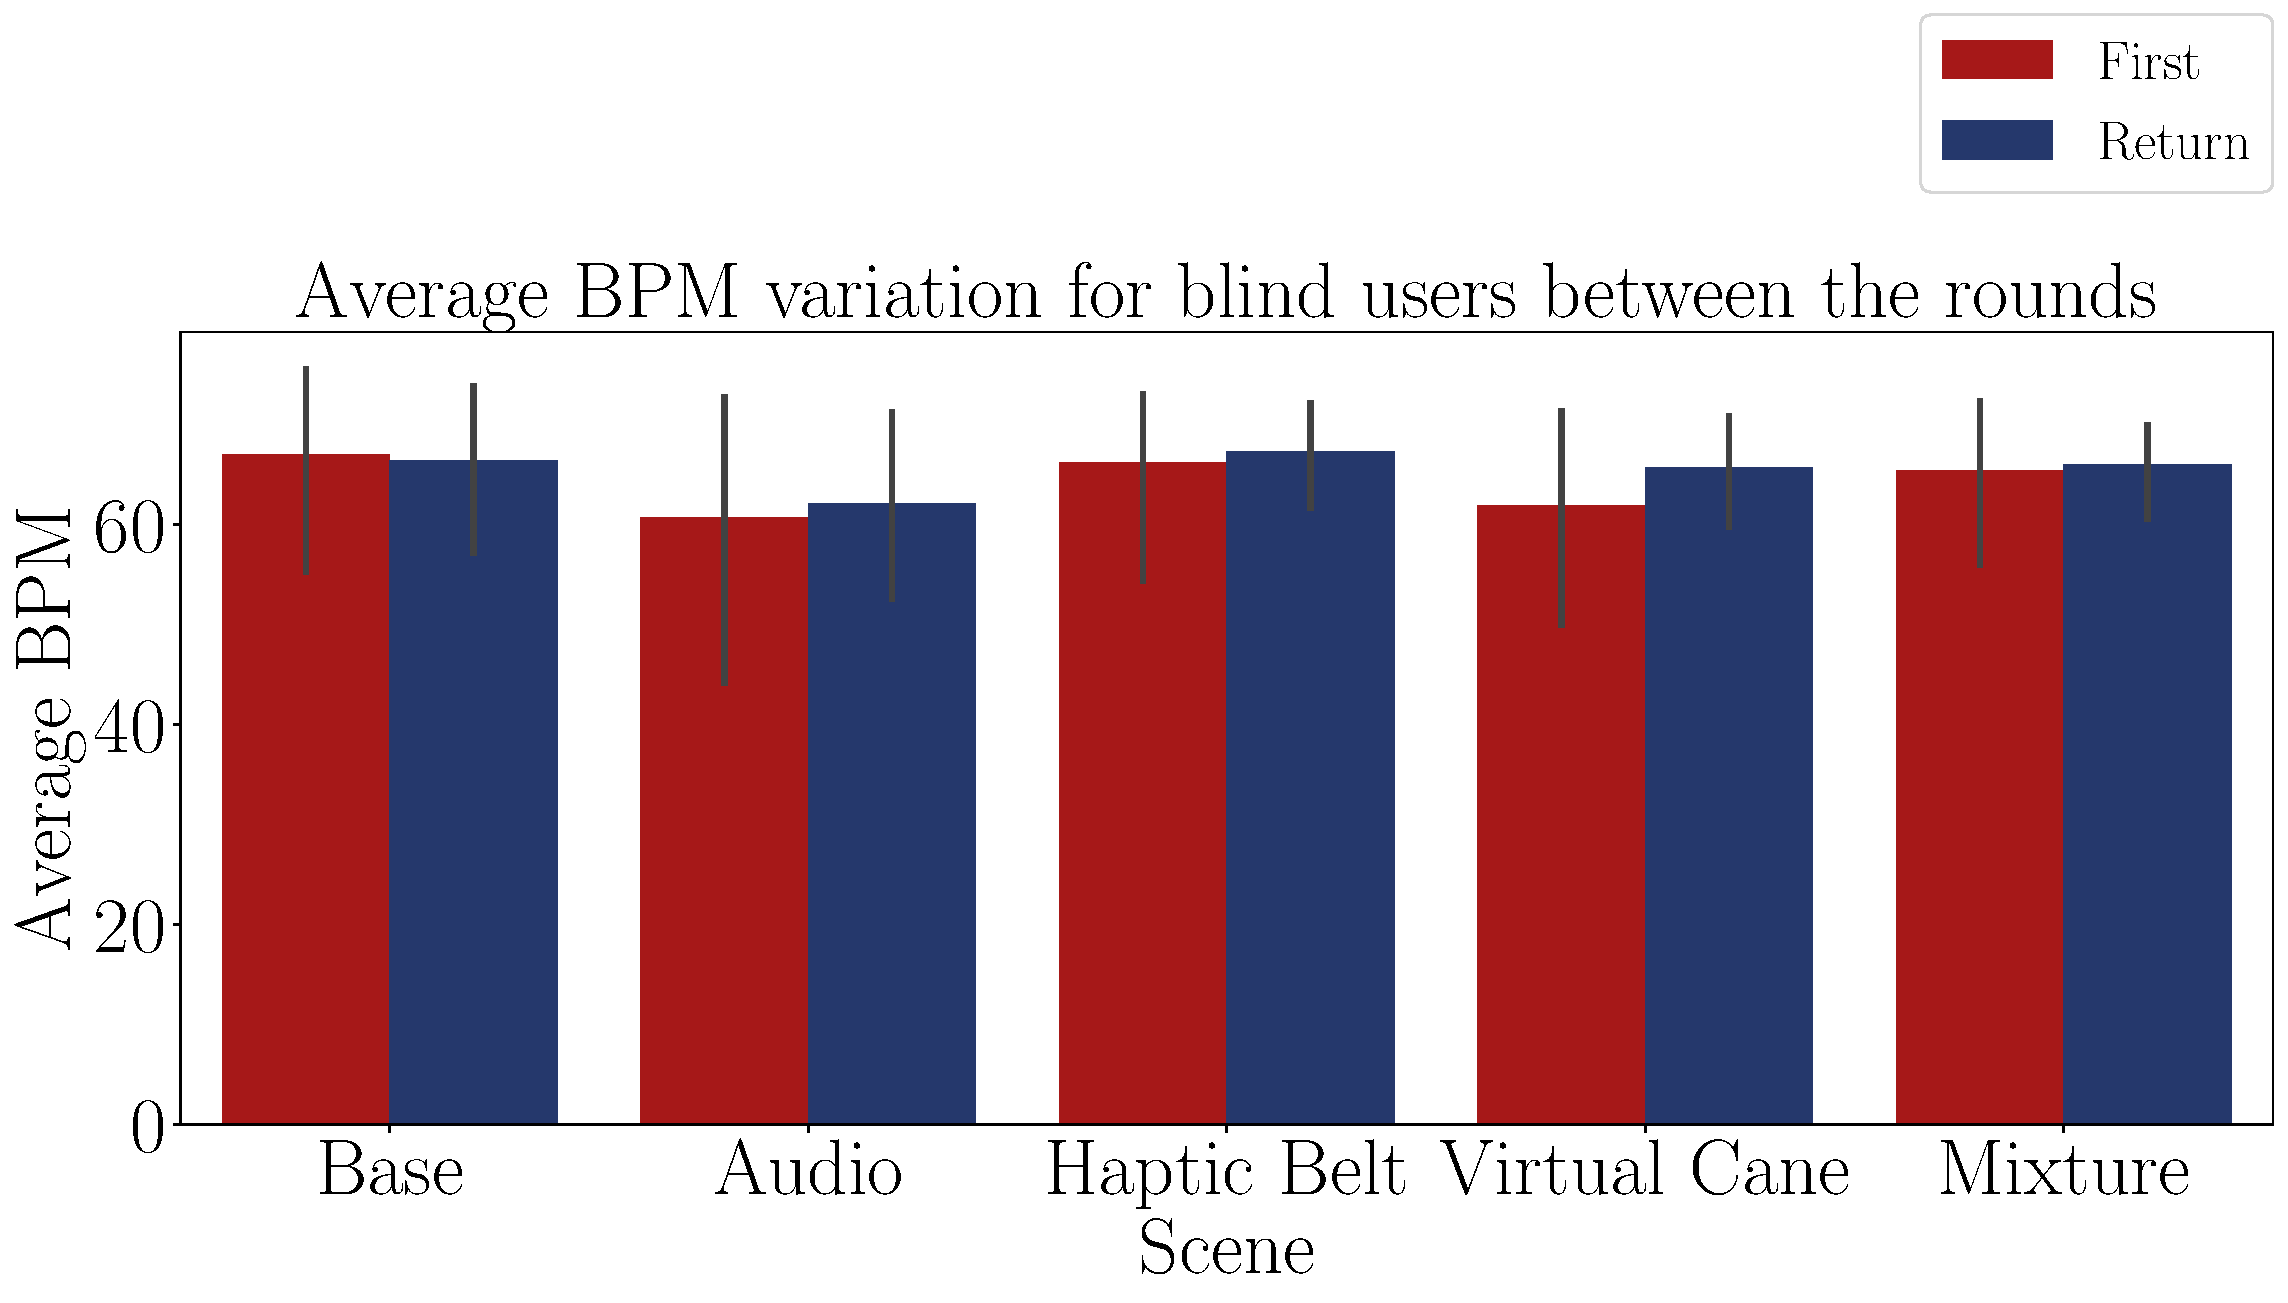
\includegraphics[width = \textwidth]{Resultados/ECG/Figuras/pdf/barplot_ecg_bpm_5_scene_blind.pdf}
    \caption{Barplot of the average BPM of the blind participants on each method.}
    \label{fig:barplot_ecg_bpm_5_scene_blind}
\end{figure}

%The Table \ref{tab:bpm_average_group_blind} show the average heartbeat frequency variation between the rounds of each group. As it was shown in the Figure \ref{fig:barplot_ecg_bpm_5_scene_blind}, only the Base method has a negative average variaton between the rounds. It is also posible to see that the Virtual Cane variation was the highest, hence it was also the highest mental workload.
% 
%
\begin{table}[!htb]
\centering
\caption{ECG average BPM  for each method of the blind participants.}
\label{tab:bpm_average_group_blind}
\begin{tabular}{lrrrrr}
\toprule
{} &   Base &  Audio & Haptic Belt & Virtual Cane & Mixture \\
Visual Condition &        &        &             &              &         \\
\midrule
Blind            &  66.69 &  61.40 &       66.68 &        63.72 &   65.65 \\
\bottomrule
\end{tabular}
\end{table}



Figures \ref{fig:boxplot_ecg_bpm_blind_scene} and \ref{fig:boxplot_ecg_bpm_blind_rounds} brings the corresponding boxplot, grouped by method and round. In both cases, it is not possible to observe significant differences among the methods or rounds.

\begin{figure}[!htb]
    \centering
    \begin{minipage}{0.45\textwidth}
        \centering
        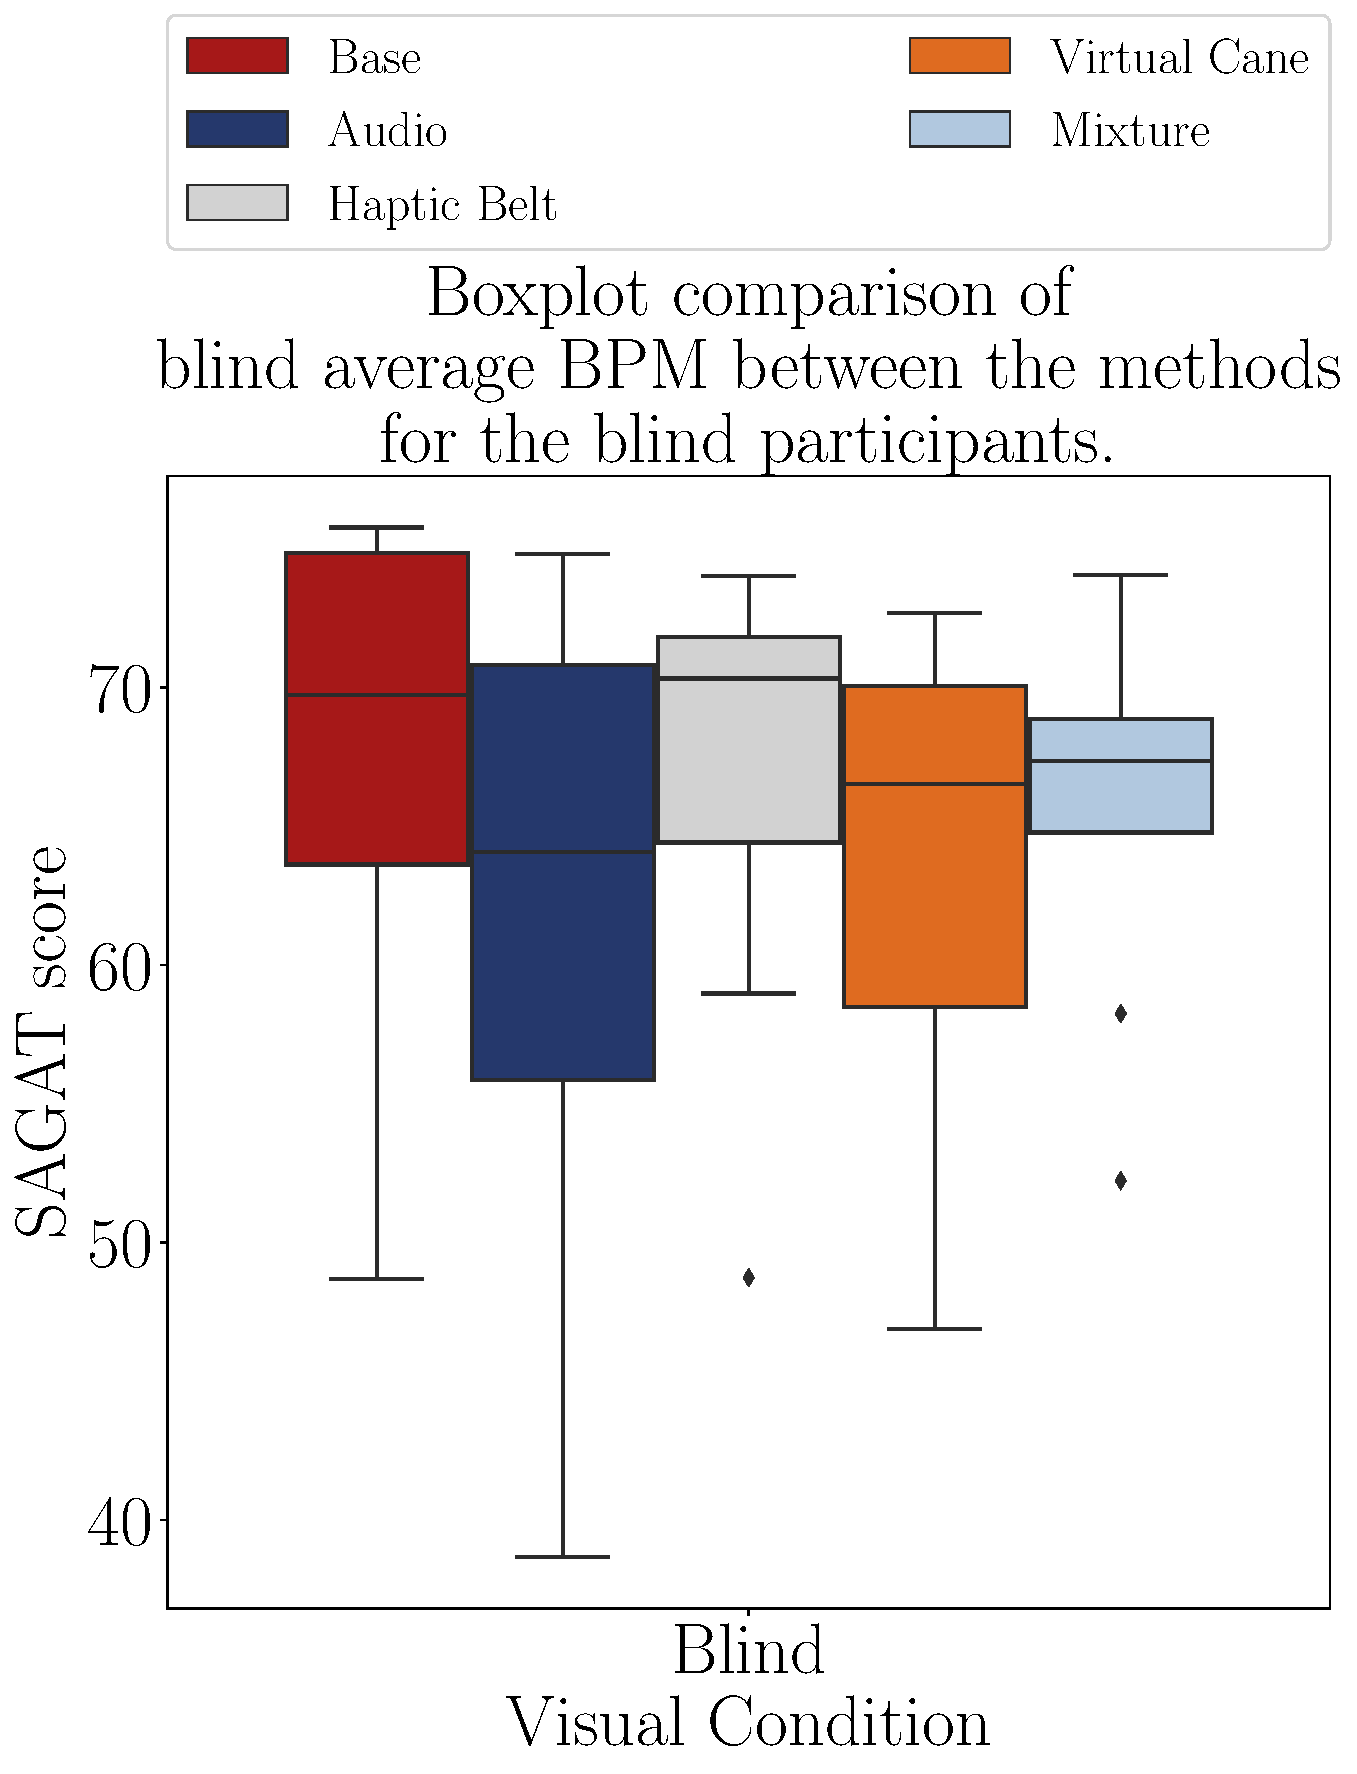
\includegraphics[width = \textwidth]{Resultados/ECG/Figuras/pdf/boxplot_ecg_bpm_blind_scene.pdf}
        \caption{Boxplot of the BPM of the blind participants grouped by the methods.}
        \label{fig:boxplot_ecg_bpm_blind_scene}
    \end{minipage}
    \begin{minipage}{0.075\textwidth}
        \hfill
    \end{minipage}
    \begin{minipage}{0.45\textwidth}
        \centering
        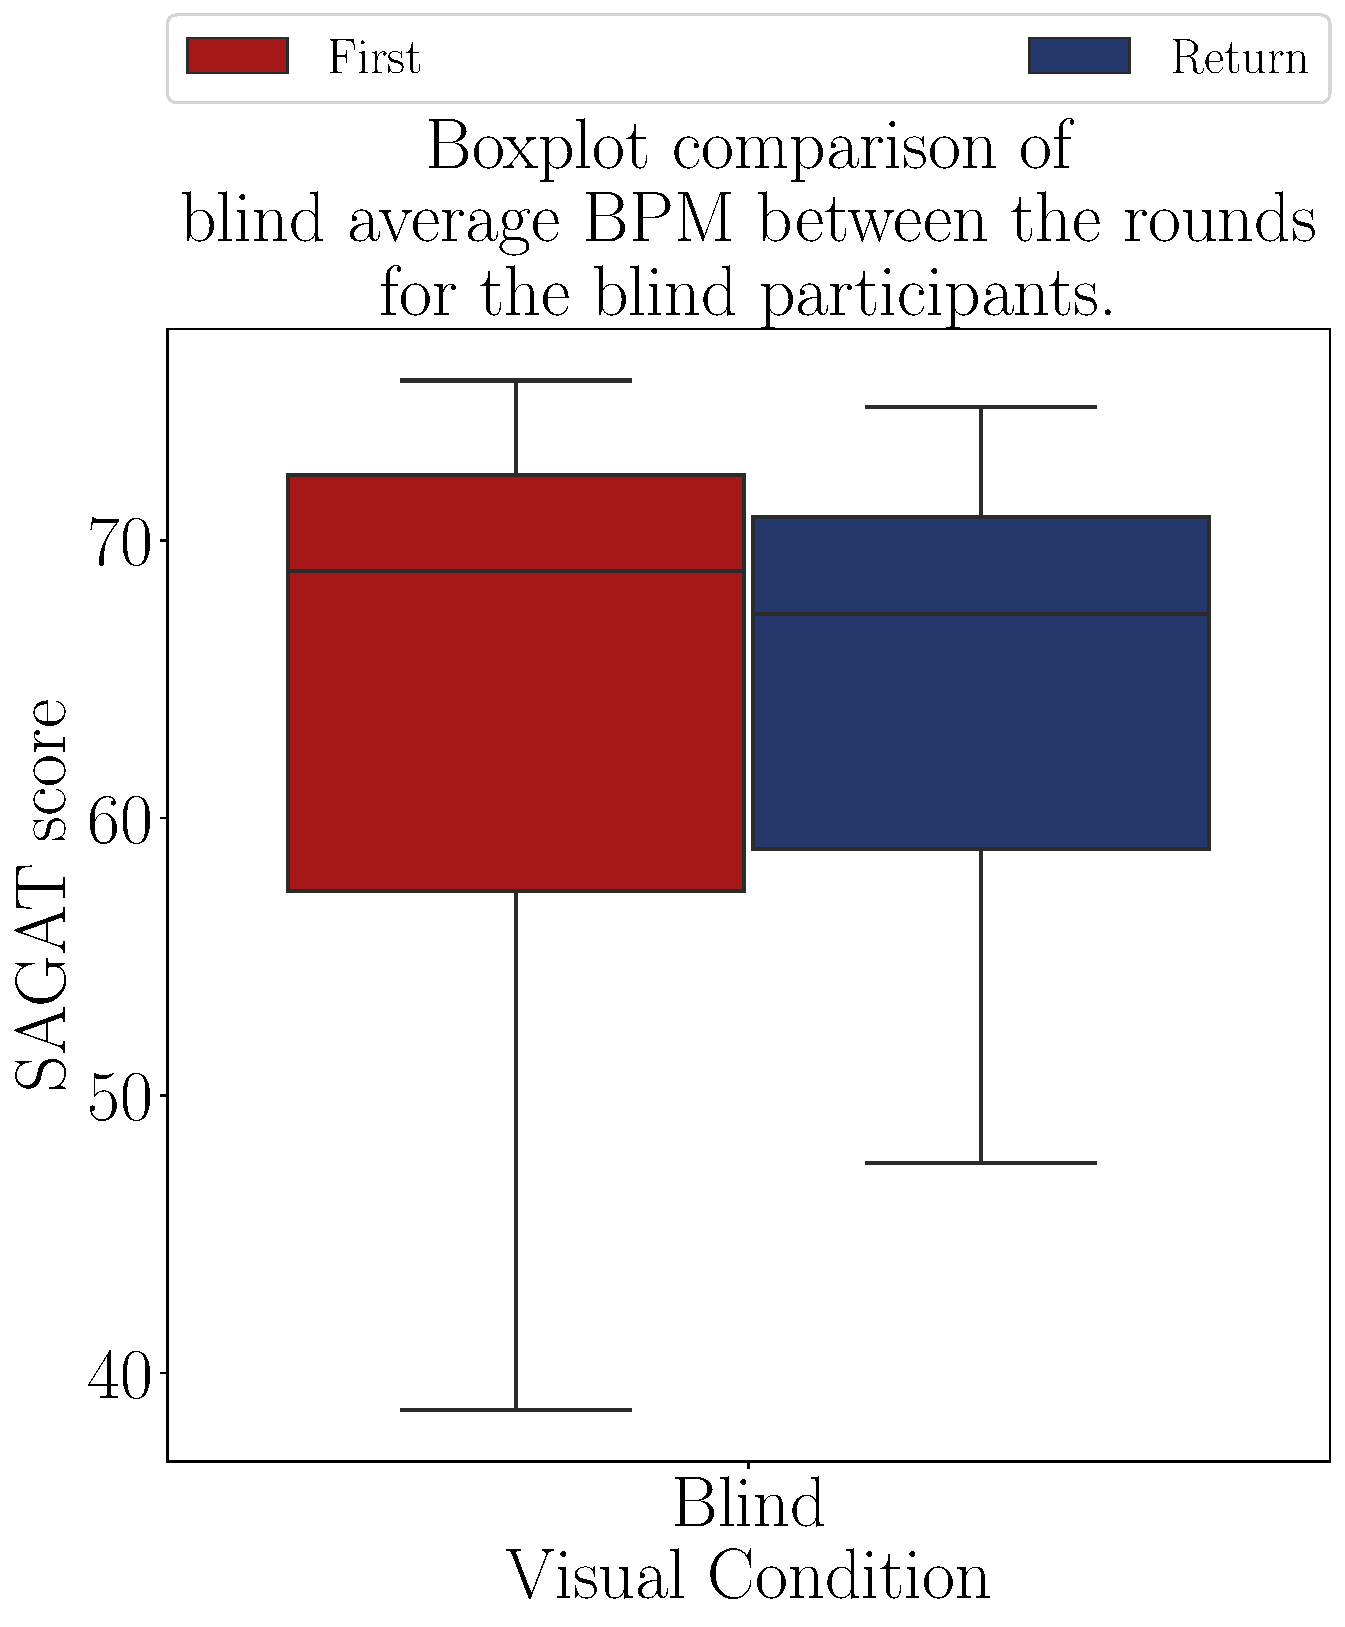
\includegraphics[width = \textwidth]{Resultados/ECG/Figuras/pdf/boxplot_ecg_bpm_blind_rounds.pdf}
        \caption{Boxplot of the BPM of the blind participants grouped by the rounds.}
        \label{fig:boxplot_ecg_bpm_blind_rounds}
    \end{minipage}
\end{figure}

Figures \ref{fig:qqplot_bpm_two_way_blind} and \ref{fig:residplot_bpm_two_way_blind} bring the QQ Plot and residual distribution. The last one shows that the participants do not have a similar variance, which may jeopardize the results of ANOVA. Considering this limitation, Table \ref{tab:bpm_table_blind} brings the p-value obtained by ANOVA, which confirmed the previous analysis, as it does not indicate a significant influence of either the guidance methods or the rounds in the participants' heart rate. 

\begin{figure}[!htb]
    \centering
    \begin{minipage}{0.45\textwidth}
        \centering
        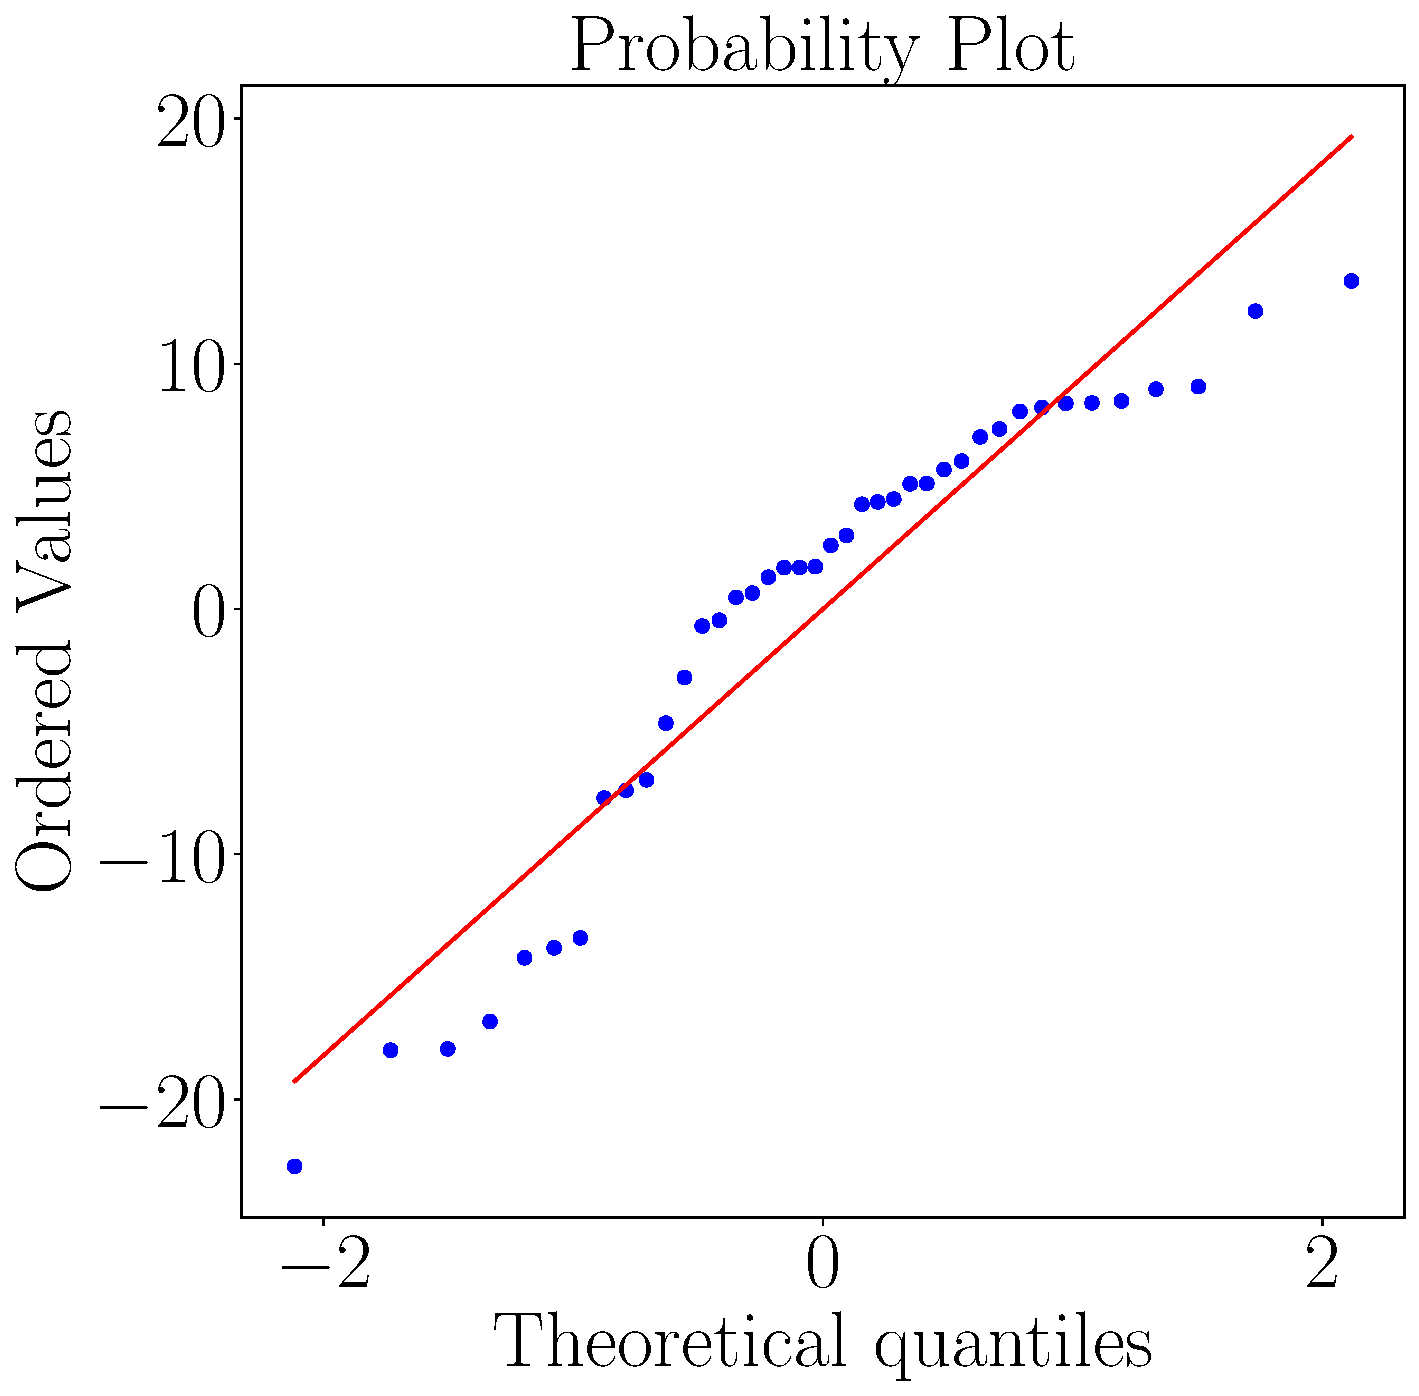
\includegraphics[width = \textwidth]{Resultados/ECG/Figuras/pdf/qqplot_bpm_two_way_blind.pdf}
        \caption{QQ plot of the BPM of the blind participants on each method.}
        \label{fig:qqplot_bpm_two_way_blind}
    \end{minipage}
    \begin{minipage}{0.075\textwidth}
        \hfill
    \end{minipage}
    \begin{minipage}{0.45\textwidth}
        \centering
        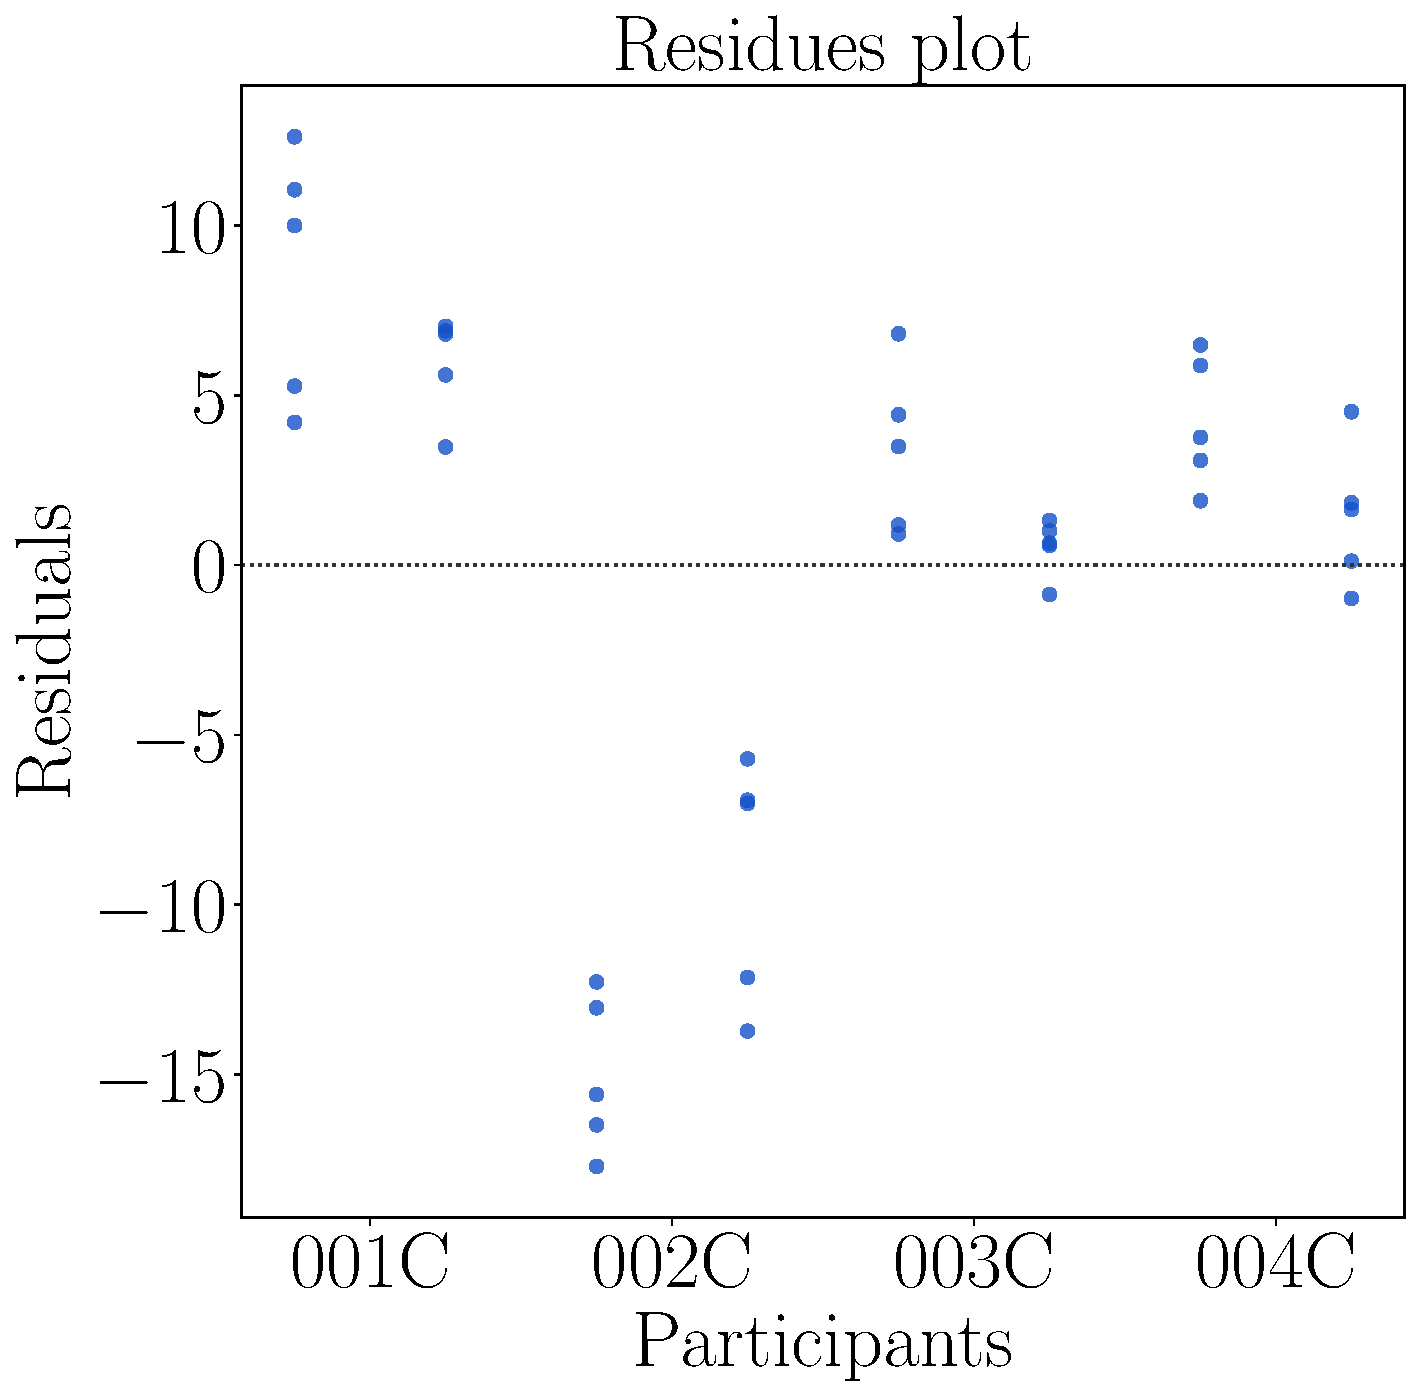
\includegraphics[width = \textwidth]{Resultados/ECG/Figuras/pdf/residplot_bpm_two_way_blind.pdf}
        \caption{Residual plot of the BPM score the blind participants on each method.}
        \label{fig:residplot_bpm_two_way_blind}
    \end{minipage}
\end{figure}


\begin{table}[!htb]
\centering
\caption{Anova p-value for the BPM on each method for blinded users.}
\label{tab:blocanova_bpm_two_way_blind}
\begin{tabular}{lrrrrr}
\toprule
          Source & P-Value \\
\midrule
    \    Methods &   0.100 \\
     \    Rounds &   0.371 \\
\    Interaction &   0.894 \\
\bottomrule
\end{tabular}
\end{table}



%\input{Resultados/ECG/Tabelas/lsd_bpm_two_way.tex}

%The Table \ref{tab:lsd_bpm_two_way} presents the conclusion of a pairwise Fisher LSD test of the blind heart rate frequency variation between all the guidance methods. The results show that the only the Base and haptic belt have simila reaction.

%\FloatBarrier

%%%%%%%%%%%%%%%%%%%%%%%%%%%%%%%%%%%%%%%%%%%%%%%%%%%%%%%%%%%%%%%%%%%%%%%%%%%%
%%%%%%%%%%%%%%%%%%%%%%%%%%%%%%%%%%%%%%%%%%%%%%%%%%%%%%%%%%%%%%%%%%%%%%%%%%%%
%%%%%%%%%%%%%%%%%%%%%%%%%%%%%%%%%%%%%%%%%%%%%%%%%%%%%%%%%%%%%%%%%%%%%%%%%%%%
%%%%%%%%%%%%%%%%%%%%%%%%%%%%%%%%%%%%%%%%%%%%%%%%%%%%%%%%%%%%%%%%%%%%%%%%%%%%
%
%
\paragraph{Analysis of the heartbeat variance (SDNN)}\mbox{}\\
%
Table \ref{tab:sdnn_table_blind} brings the value of the second variable extracted from the ECG: SDNN, the standard deviation of the interbeat interval. Different to the heart rate frequency, if the variation between the First and the Return round is negative, it means that the user had an increase on his/her mental workload and vice-versa. Similar to what is observed for the BPM, it is not possible to draw a pattern from this data. The participants had increased or decreased their heart rate with different methods.


\begin{table}[!htb]
\centering
\caption{Average SDNN of the blind participants during the each round and method [ms].}
\label{tab:sdnn_table_blind}
\begin{tabular}{llrrrrr}
\toprule
     &        &    Base &   Audio &  \begin{tabular}[c]{@{}l@{}}Haptic\\ Belt\end{tabular} &  \begin{tabular}[c]{@{}l@{}}Virtual\\ Cane\end{tabular} &  Mixture \\
Participant & Round &         &         &                                                        &                                                         &          \\
\midrule
001C & First &  81.292 & 107.061 &                                                124.737 &                                                 163.968 &  129.054 \\
     & Return & 120.719 & 130.885 &                                                131.590 &                                                 157.589 &  124.786 \\
002C & First &  73.761 &  98.863 &                                                 81.140 &                                                  33.977 &   79.289 \\
     & Return & 108.940 &  49.627 &                                                 42.815 &                                                 114.057 &  107.545 \\
003C & First &  36.870 &  38.325 &                                                 35.101 &                                                  42.392 &   43.692 \\
     & Return &  52.750 &  41.196 &                                                 44.256 &                                                  42.602 &   46.145 \\
004C & First &  70.728 &  86.827 &                                                 62.560 &                                                  85.900 &   70.472 \\
     & Return &  71.950 &  74.895 &                                                 70.017 &                                                  66.089 &  104.040 \\
\bottomrule
\end{tabular}
\end{table}



The barplot of Figure \ref{fig:barplot_ecg_sdnn_5_scene_blind} shows the average SDNN for each method. It is possible to notice that some methods are associated with an increase in the SDNN between the rounds, while others present a slight decrease.

\begin{figure}[!htb]
    \centering
    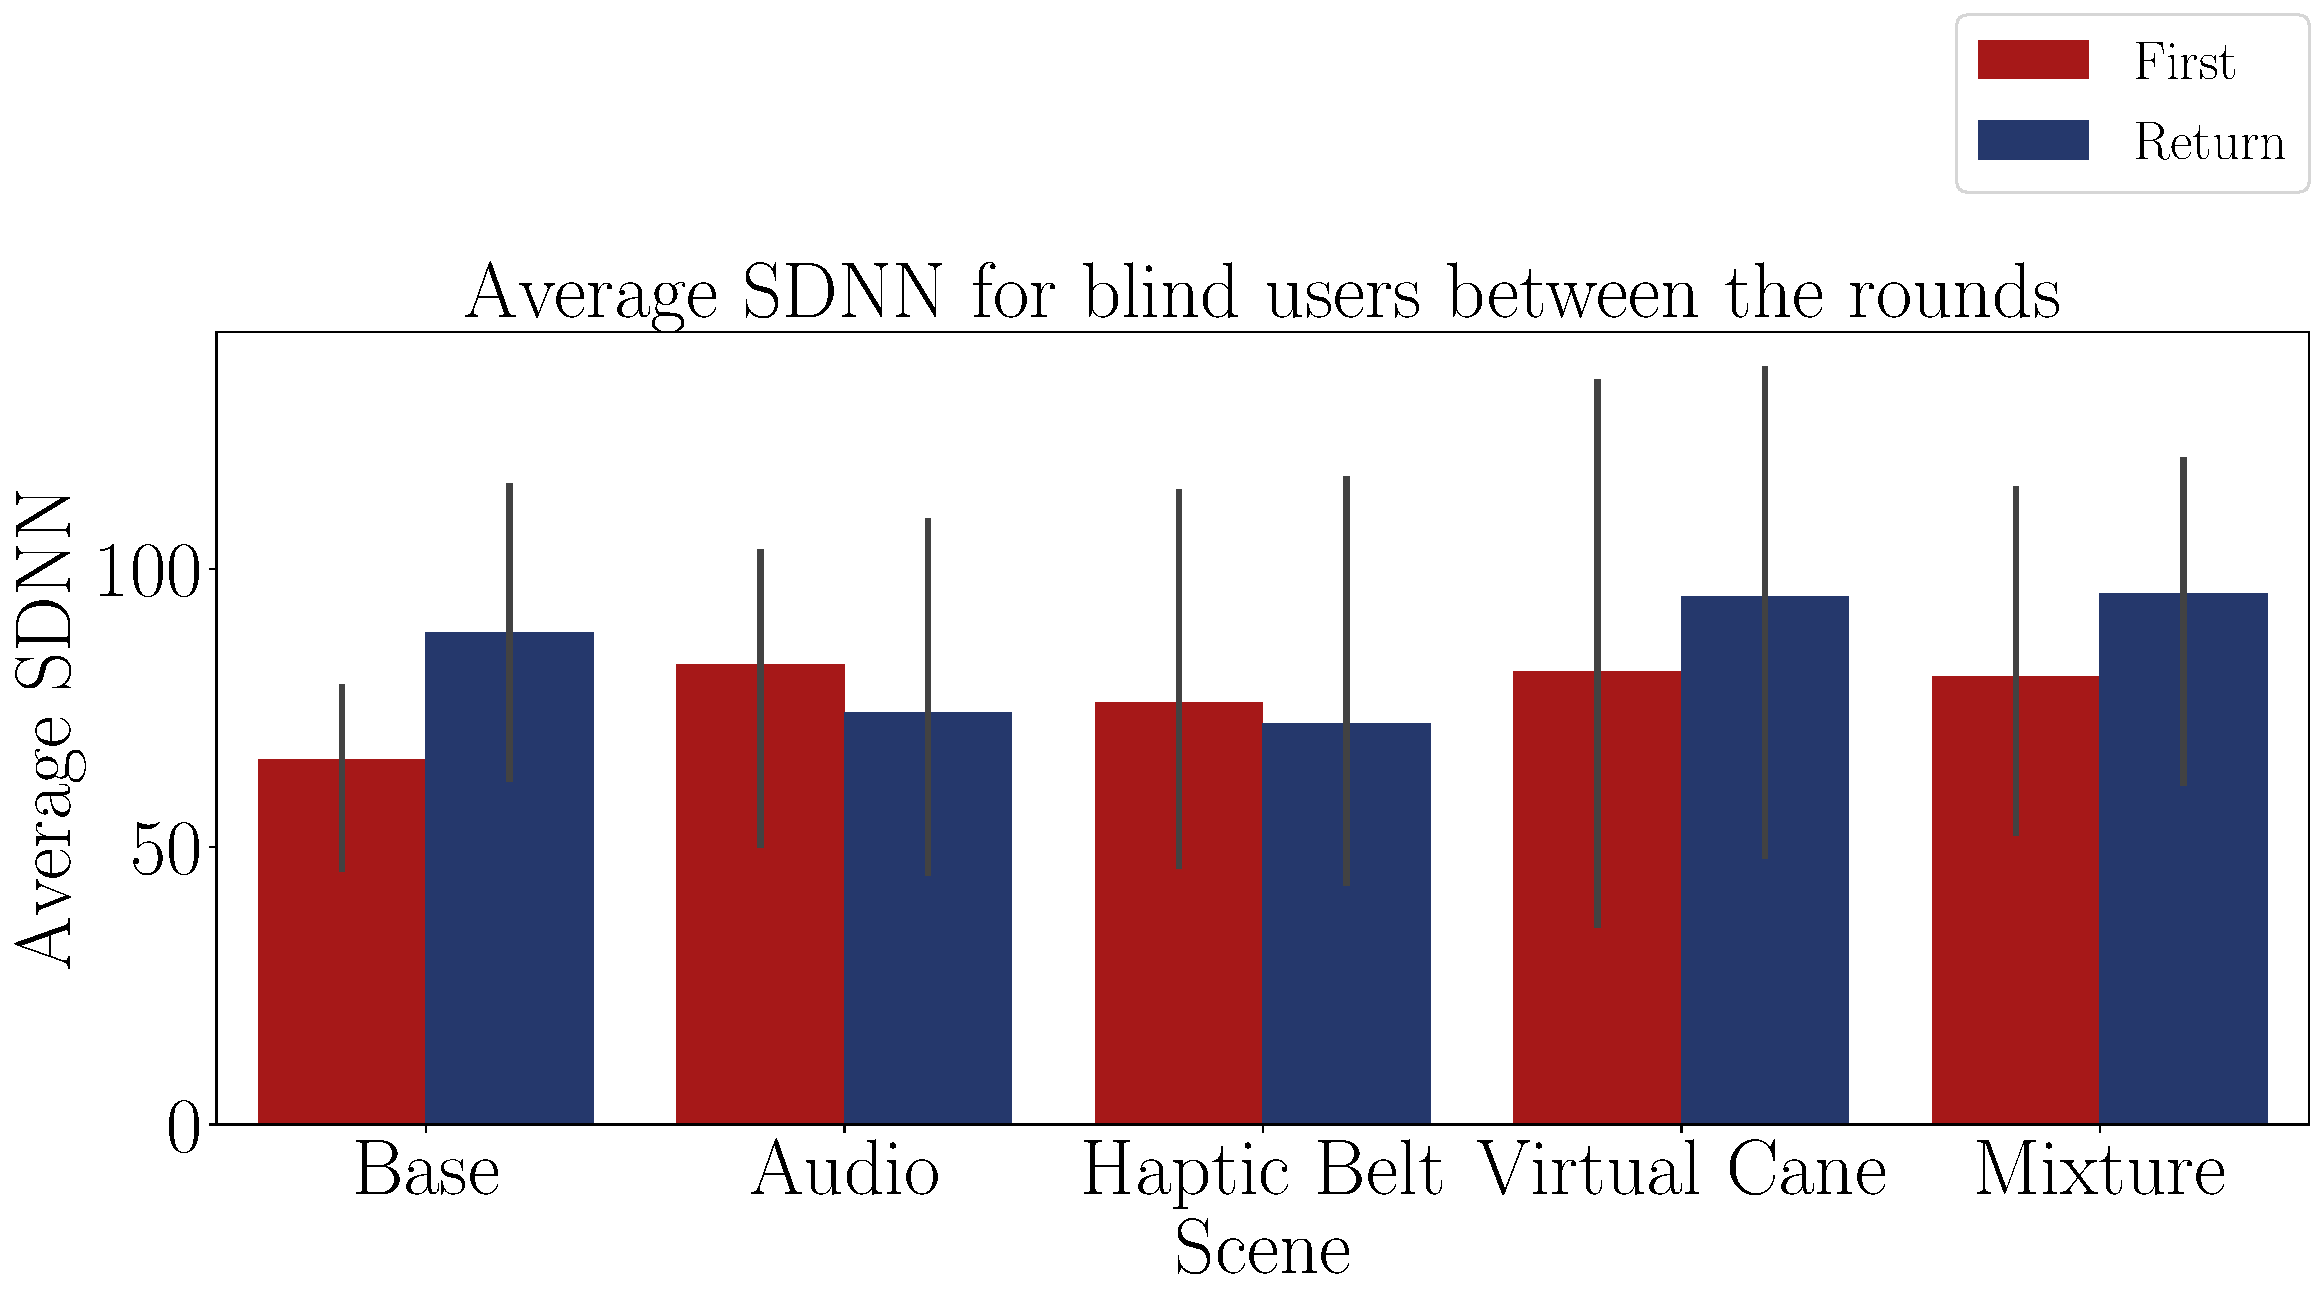
\includegraphics[width = \textwidth]{Resultados/ECG/Figuras/pdf/barplot_ecg_sdnn_5_scene_blind.pdf}
    \caption{Barplot of the average SDNN of the blind participants on each method.}
    \label{fig:barplot_ecg_sdnn_5_scene_blind}
\end{figure}

%The Table \ref{tab:sdnn_average_group_blind} presents the average SDNN variation between the rounds. It shows that only the audio and the haptic belt methods shown a increase in the mental workload.
%
%
\begin{table}[!htb]
\centering
\caption{ECG average SDNN for each method of the blind participants.}
\label{tab:sdnn_average_group_blind}
\begin{tabular}{lrrrrr}
\toprule
{} &   Base &  Audio & Haptic Belt & Virtual Cane & Mixture \\
Visual Condition &        &        &             &              &         \\
\midrule
Blind            &  77.13 &  78.46 &       74.03 &        88.32 &   88.13 \\
\bottomrule
\end{tabular}
\end{table}



Figure \ref{fig:boxplot_ecg_sdnn_blind_scene} and Figure \ref{fig:boxplot_ecg_sdnn_blind_rounds} bring the SDNN barplot grouped by the methods and the rounds. There is a slight tendency among the participants to increase the heartbeat in the return round.

\begin{figure}[!htb]
    \centering
    \begin{minipage}{0.45\textwidth}
        \centering
        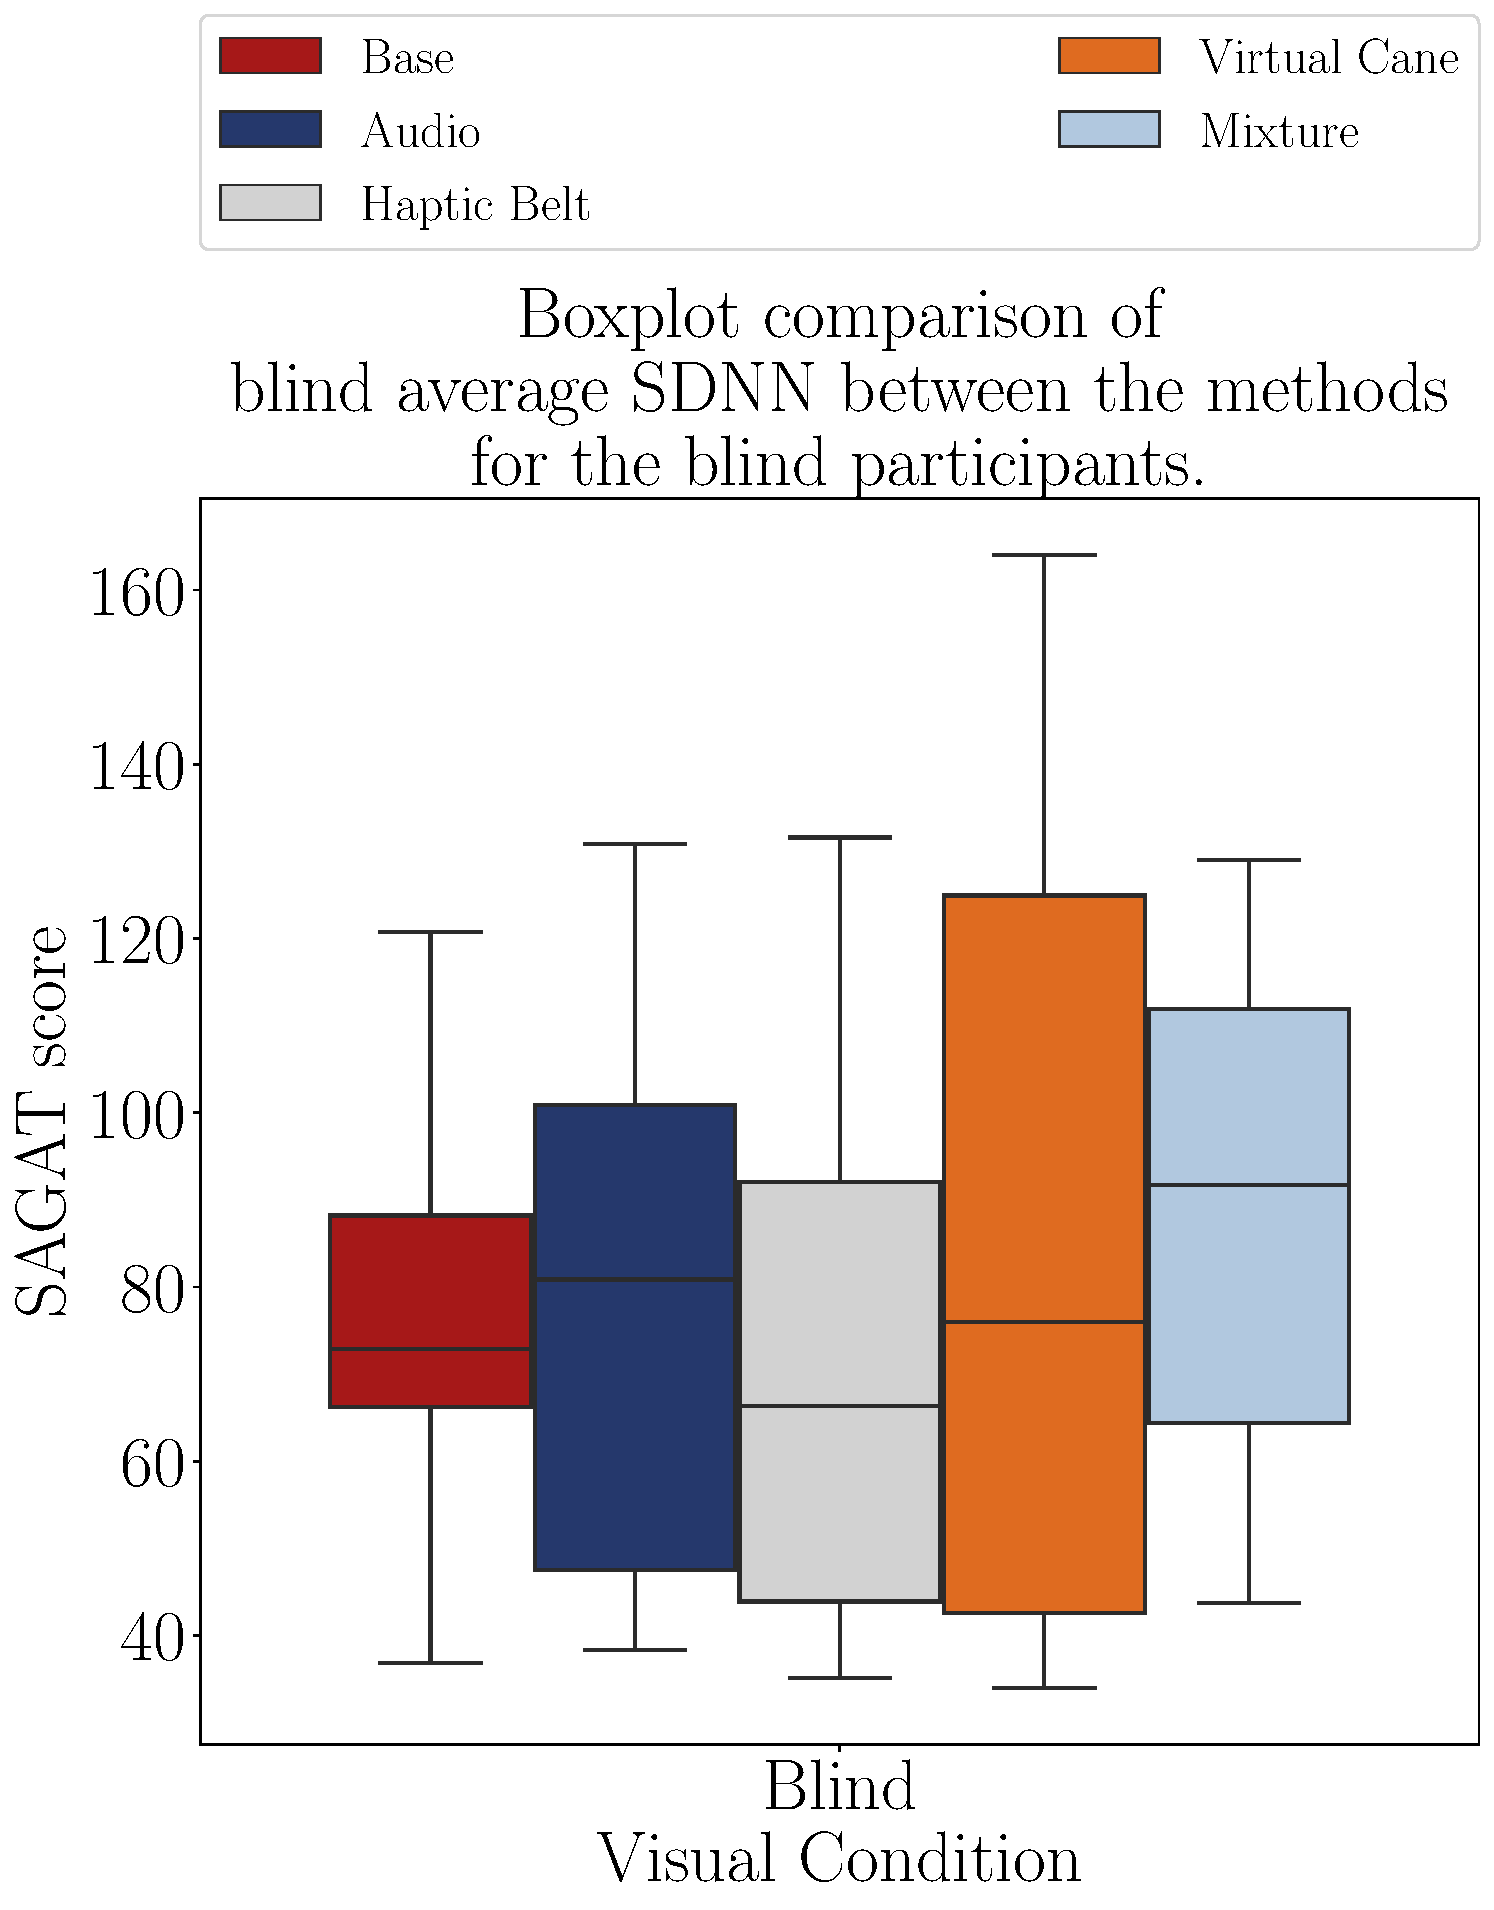
\includegraphics[width = \textwidth]{Resultados/ECG/Figuras/pdf/boxplot_ecg_sdnn_blind_scene.pdf}
        \caption{Boxplot of the SDNN of the blind participants grouped by the methods.}
        \label{fig:boxplot_ecg_sdnn_blind_scene}
    \end{minipage}
    \begin{minipage}{0.075\textwidth}
        \hfill
    \end{minipage}
    \begin{minipage}{0.45\textwidth}
        \centering
        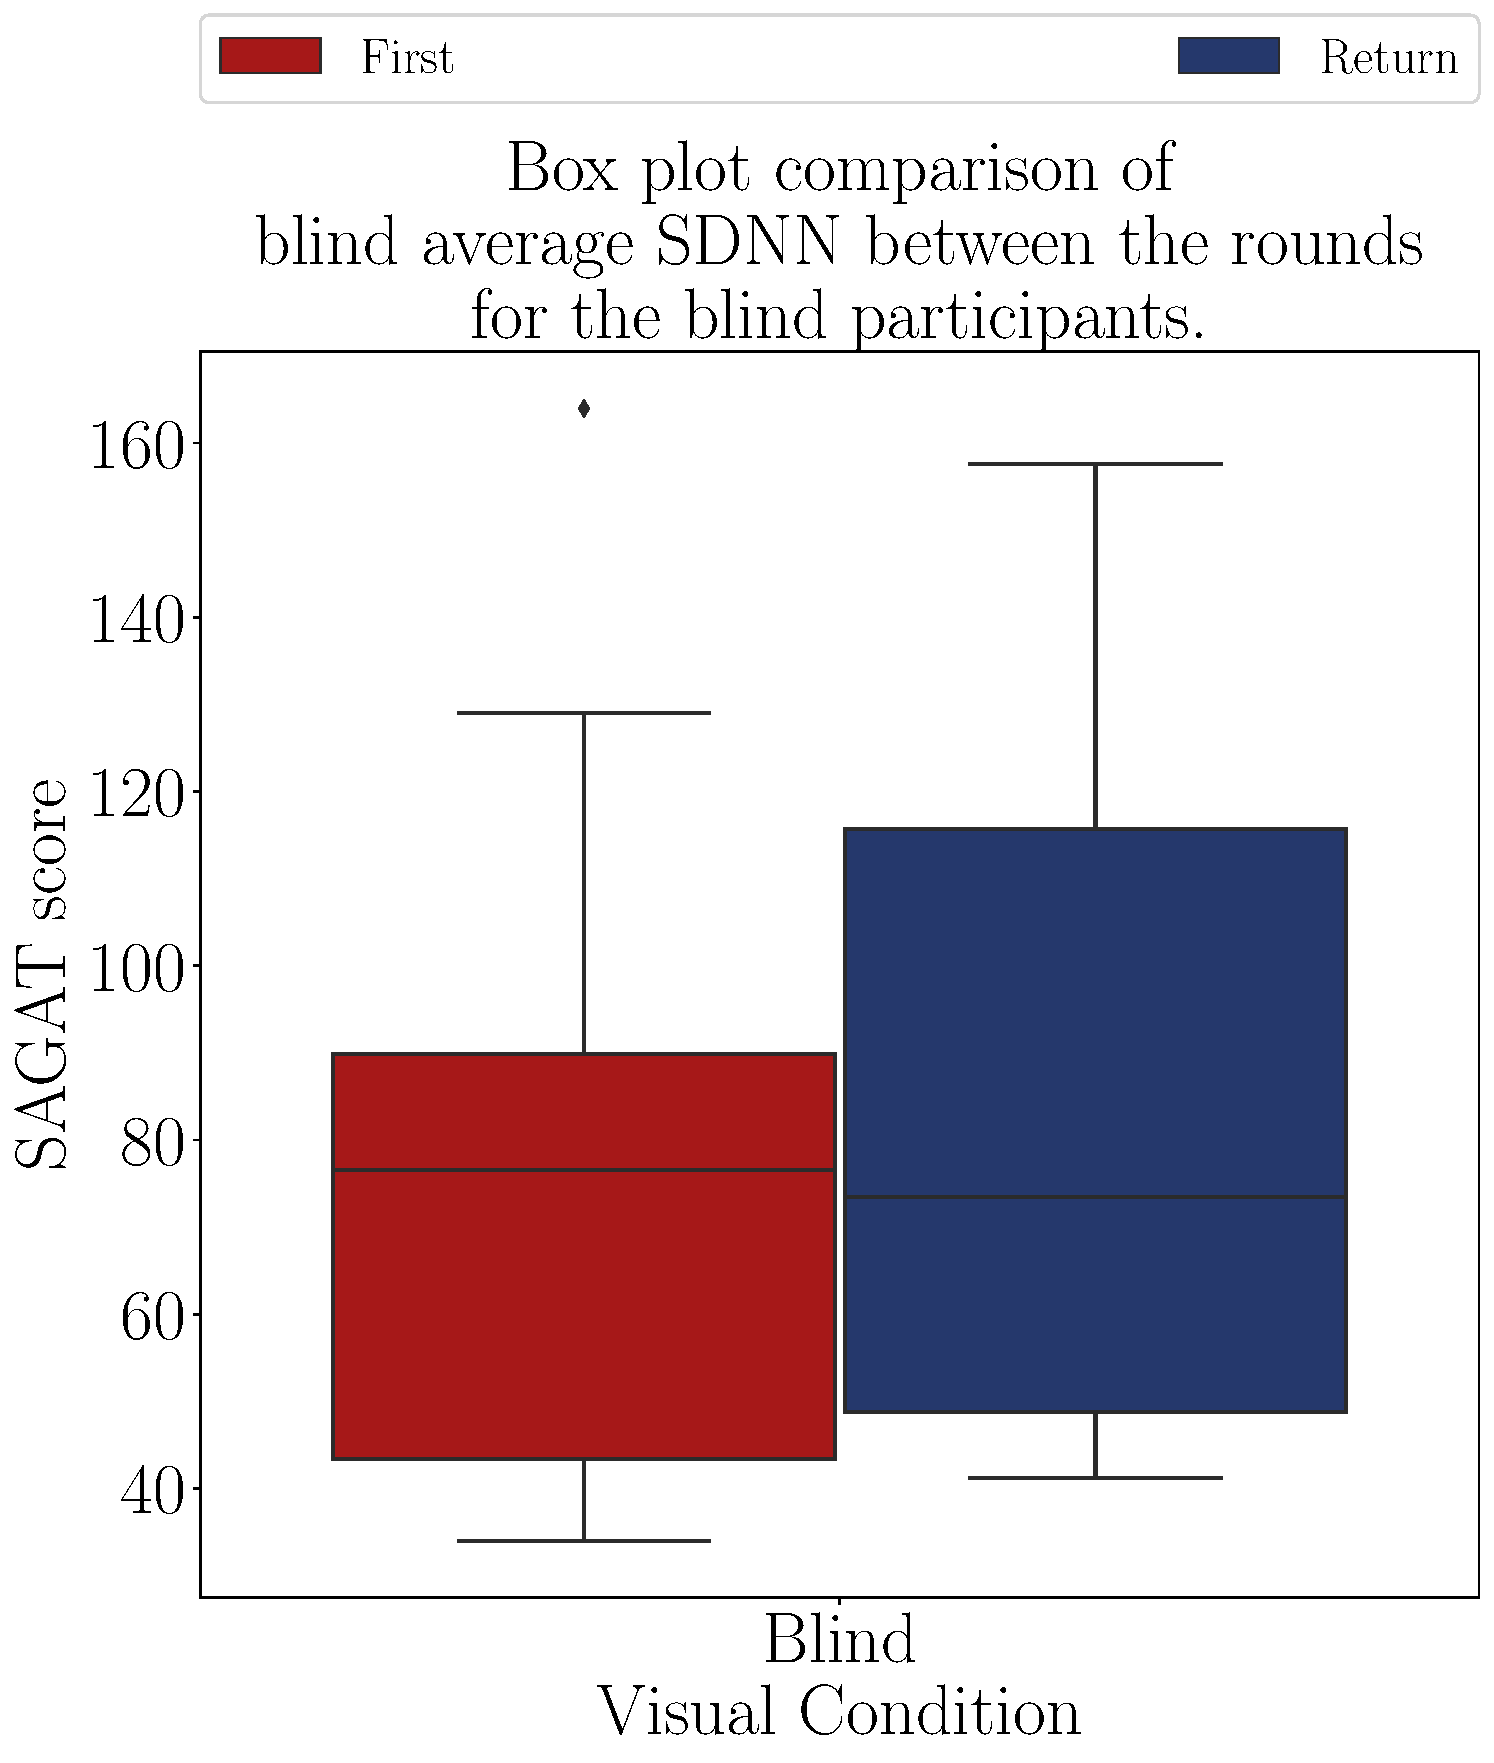
\includegraphics[width = \textwidth]{Resultados/ECG/Figuras/pdf/boxplot_ecg_sdnn_blind_rounds.pdf}
        \caption{Boxplot of the SDNN of the blind participants grouped by the rounds.}
        \label{fig:boxplot_ecg_sdnn_blind_rounds}
    \end{minipage}
\end{figure}


Figures \ref{fig:qqplot_sdnn_two_way_blind} and \ref{fig:residplot_sdnn_two_way_blind} bring the QQ Plot and residual distribution. In this case, the residual distribution is more uniform than in Figure \ref{fig:residplot_bpm_two_way_blind}. The ANOVA results are presented in Table \ref{tab:blocdanova_sdnn_two_way_blind} and do not confirm any influence of the methods nor the rounds on the ECG heart rate variance.

\begin{figure}[!htb]
    \centering
    \begin{minipage}{0.45\textwidth}
        \centering
        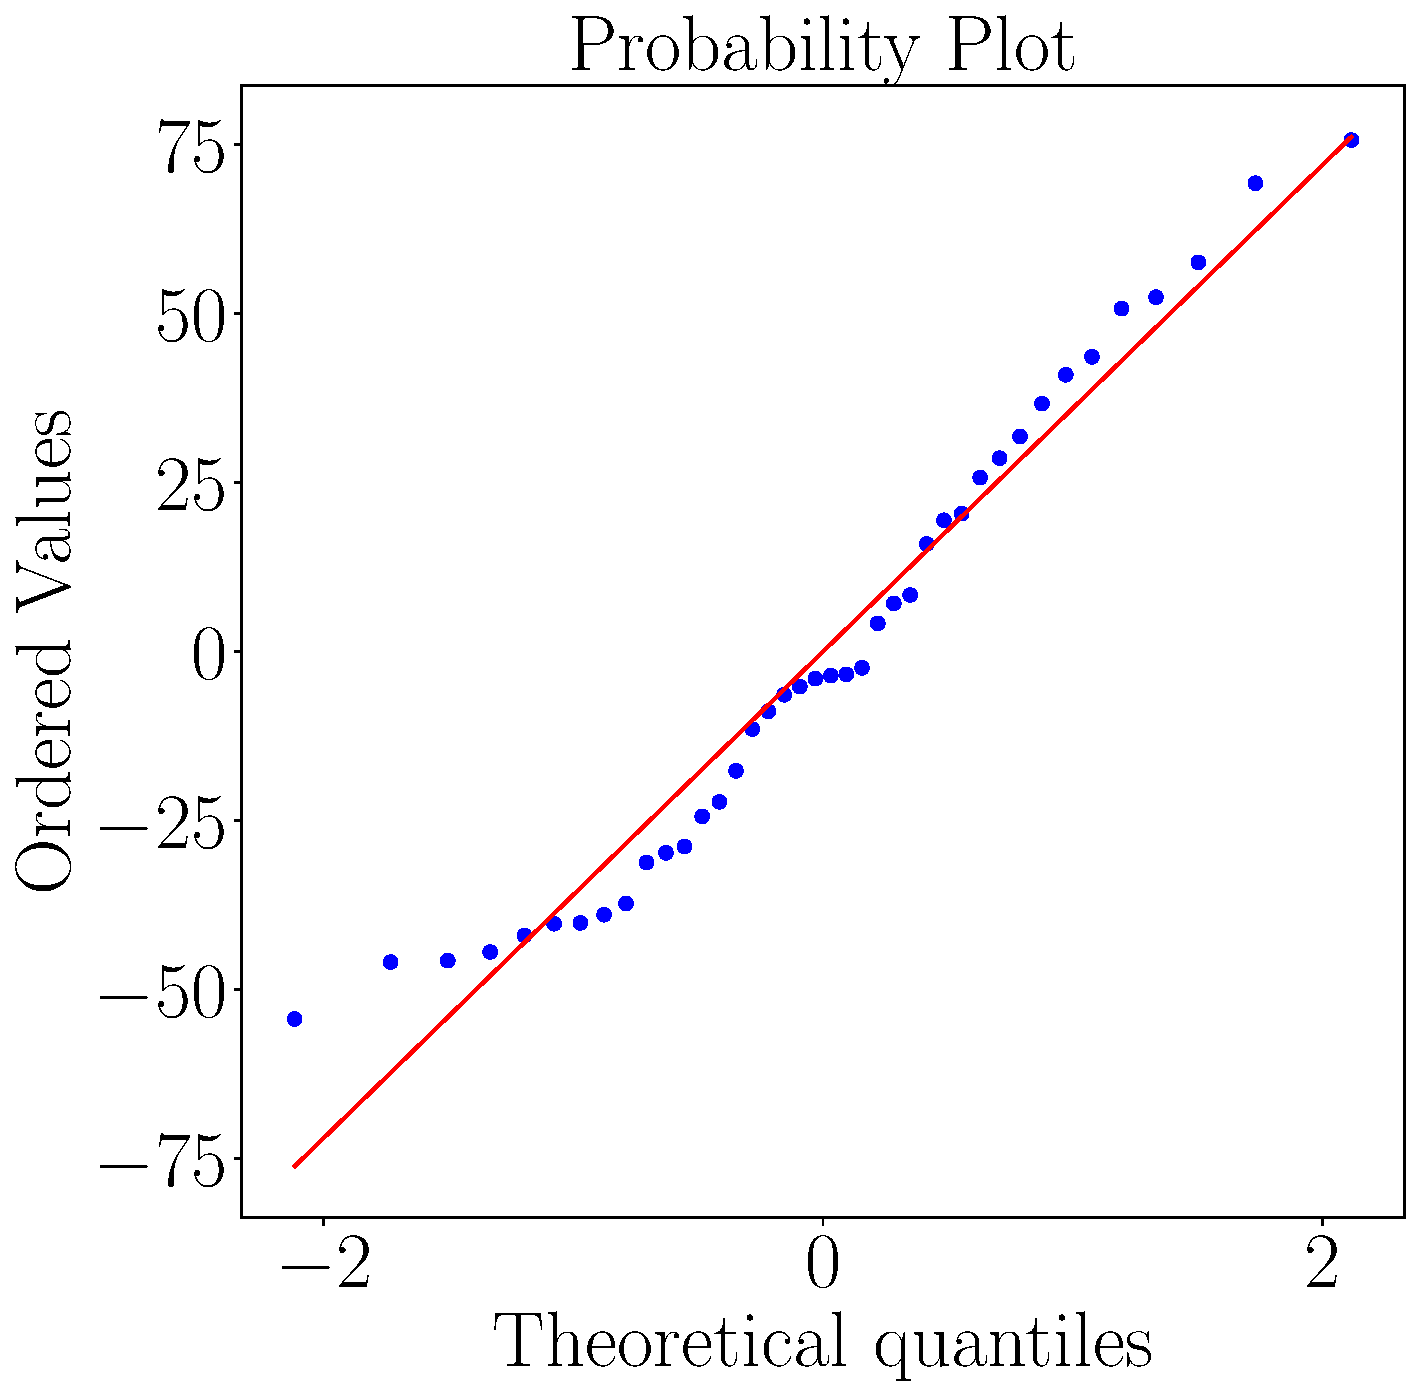
\includegraphics[width = \textwidth]{Resultados/ECG/Figuras/pdf/qqplot_sdnn_two_way_blind.pdf}
        \caption{QQ plot of the SDNN of the blind participants on each method.}
        \label{fig:qqplot_sdnn_two_way_blind}
    \end{minipage}
    \begin{minipage}{0.075\textwidth}
        \hfill
    \end{minipage}
    \begin{minipage}{0.45\textwidth}
        \centering
        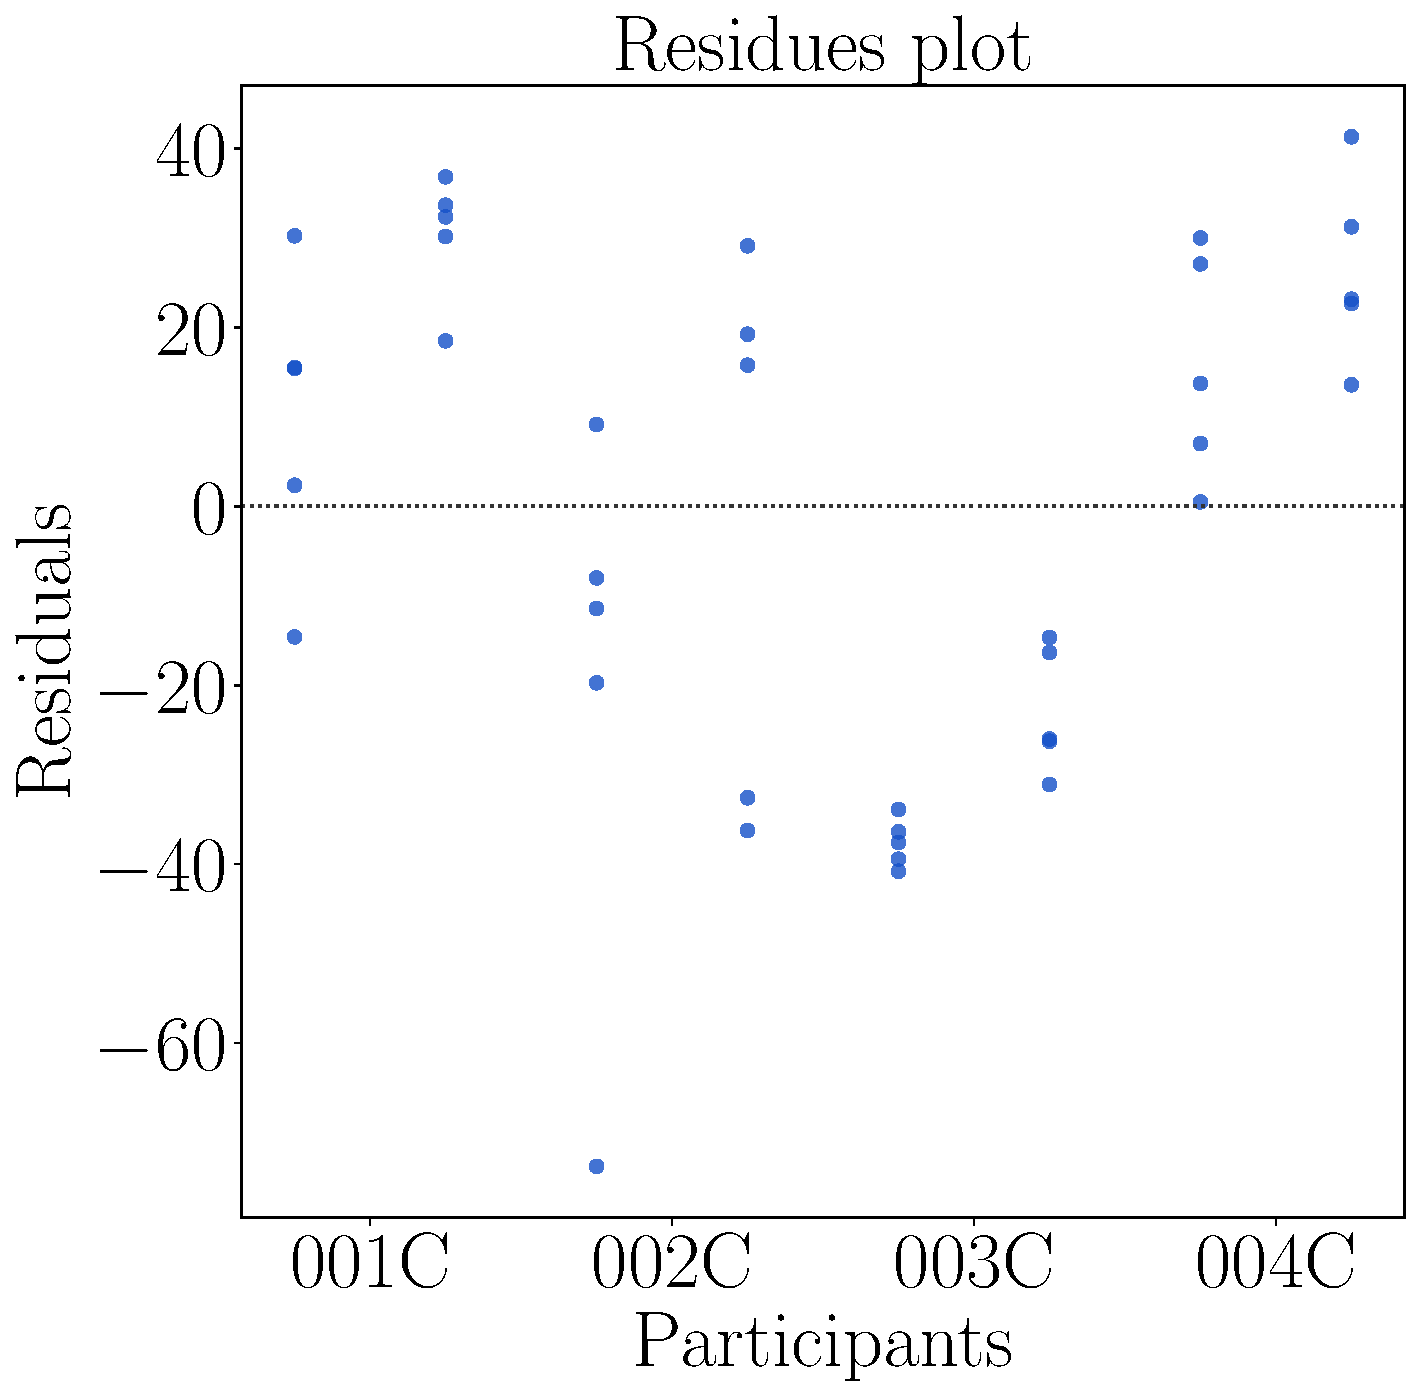
\includegraphics[width = \textwidth]{Resultados/ECG/Figuras/pdf/residplot_sdnn_two_way_blind.pdf}
        \caption{Residual plot of the SDNN of the blind participants on each method.}
        \label{fig:residplot_sdnn_two_way_blind}
    \end{minipage}
\end{figure}


\begin{table}[H]
\centering
\caption{Anova p-value for the average SDNN on each method for blinded users.}
\label{tab:blocdanova_sdnn_two_way_blind}
\begin{tabular}{lrrrrr}
\toprule
          Source & P-Value \\
\midrule
    \    Methods &   0.486 \\
     \    Rounds &   0.223 \\
\    Interaction &   0.473 \\
\bottomrule
\end{tabular}
\end{table}



\FloatBarrier

\subsubsection{Galvanic skin response and temperature data;}
\label{subsubsec:results_gsr_temp_1}

The GSR analysis is based on the signal's average level. Each experiment's round is compared to the participant baseline collected before the experiment. The GSR sensor was worn on the left hand for right-handed participant and on the right hand for left-handed participants. One of the blind participants had the GSR sensor removed during the experiment because it was not appropriately fixed.

Table \ref{tab:gsr_table_blind} presents the GSR average values for the three remaining participants. If the variation between the round and the Baseline is positive, it means that the user had an increase on his/her Mental Workload or stress. For all the participants, the baseline was smaller than the values obtained during the experiment, as expected. Moreover, in most cases, the skin conductance has risen from the first to the return, indicating an increase in the mental workload.


\begin{table}[!htb]
\centering
\caption{Average GSR felled by the blind participants [$\mu$S].}
\label{tab:gsr_table_blind}
\begin{tabular}{lllrrrrrr}
\toprule
     &        & Baseline &  Base & Audio & \begin{tabular}[c]{@{}l@{}}Haptic\\ Belt\end{tabular} & \begin{tabular}[c]{@{}l@{}}Virtual\\ Cane\end{tabular} & Mixture \\
Participant & Round &          &       &       &                                                       &                                                        &         \\
\midrule
001C & First &     0.37 &  0.48 &  1.03 &                                                  3.14 &                                                   3.79 &    3.90 \\
     & Return &          &  0.83 &  1.58 &                                                  2.81 &                                                   4.04 &    4.57 \\
003C & First &     0.30 &  0.56 &  0.56 &                                                  0.62 &                                                   0.85 &    1.09 \\
     & Return &          &  0.62 &  0.63 &                                                  0.65 &                                                   0.92 &    1.06 \\
004C & First &     1.24 &  2.34 &  3.07 &                                                  3.49 &                                                   2.28 &    2.23 \\
     & Return &          &  2.57 &  2.95 &                                                  3.20 &                                                   2.21 &    2.24 \\
\bottomrule
\end{tabular}
\end{table}



Table \ref{tab:gsr_var_blind} brings the percentual increase in the GSR average compared to the baseline value. Figure \ref{fig:barplot_gsr_avg_5_scene_blind} shows the corresponding barplot. The presence of a haptic device causes an increase in the skin conductance, hence its mental workload. Also, it is possible to observe the increase in GSR average between the two rounds, except for the haptic belt.


\begin{table}[!htb]
\centering
\caption{Average GSR variation in relation to the baseline in each round of the blind participants [$\mu$S].}
\label{tab:gsr_var_blind}
\begin{tabular}{lllrrrrrr}
\toprule
     &        &      Base &     Audio & \begin{tabular}[c]{@{}l@{}}Haptic\\ Belt\end{tabular} & \begin{tabular}[c]{@{}l@{}}Virtual\\ Cane\end{tabular} &    Mixture \\
Participant & Round &           &           &                                                       &                                                        &            \\
\midrule
001C & First &   30.58\% &  176.54\% &                                              746.10\% &                                               920.72\% &   951.71\% \\
     & Return &  125.29\% &  327.42\% &                                              656.99\% &                                               988.93\% &  1132.39\% \\
003C & First &   85.36\% &   84.23\% &                                              104.19\% &                                               182.35\% &   258.80\% \\
     & Return &  105.34\% &  109.23\% &                                              112.95\% &                                               202.35\% &   249.72\% \\
004C & First &   89.62\% &  148.53\% &                                              182.84\% &                                                84.33\% &    80.69\% \\
     & Return &  108.22\% &  138.64\% &                                              159.00\% &                                                78.73\% &    81.61\% \\
\bottomrule
\end{tabular}
\end{table}



\begin{figure}[!htb]
    \centering
    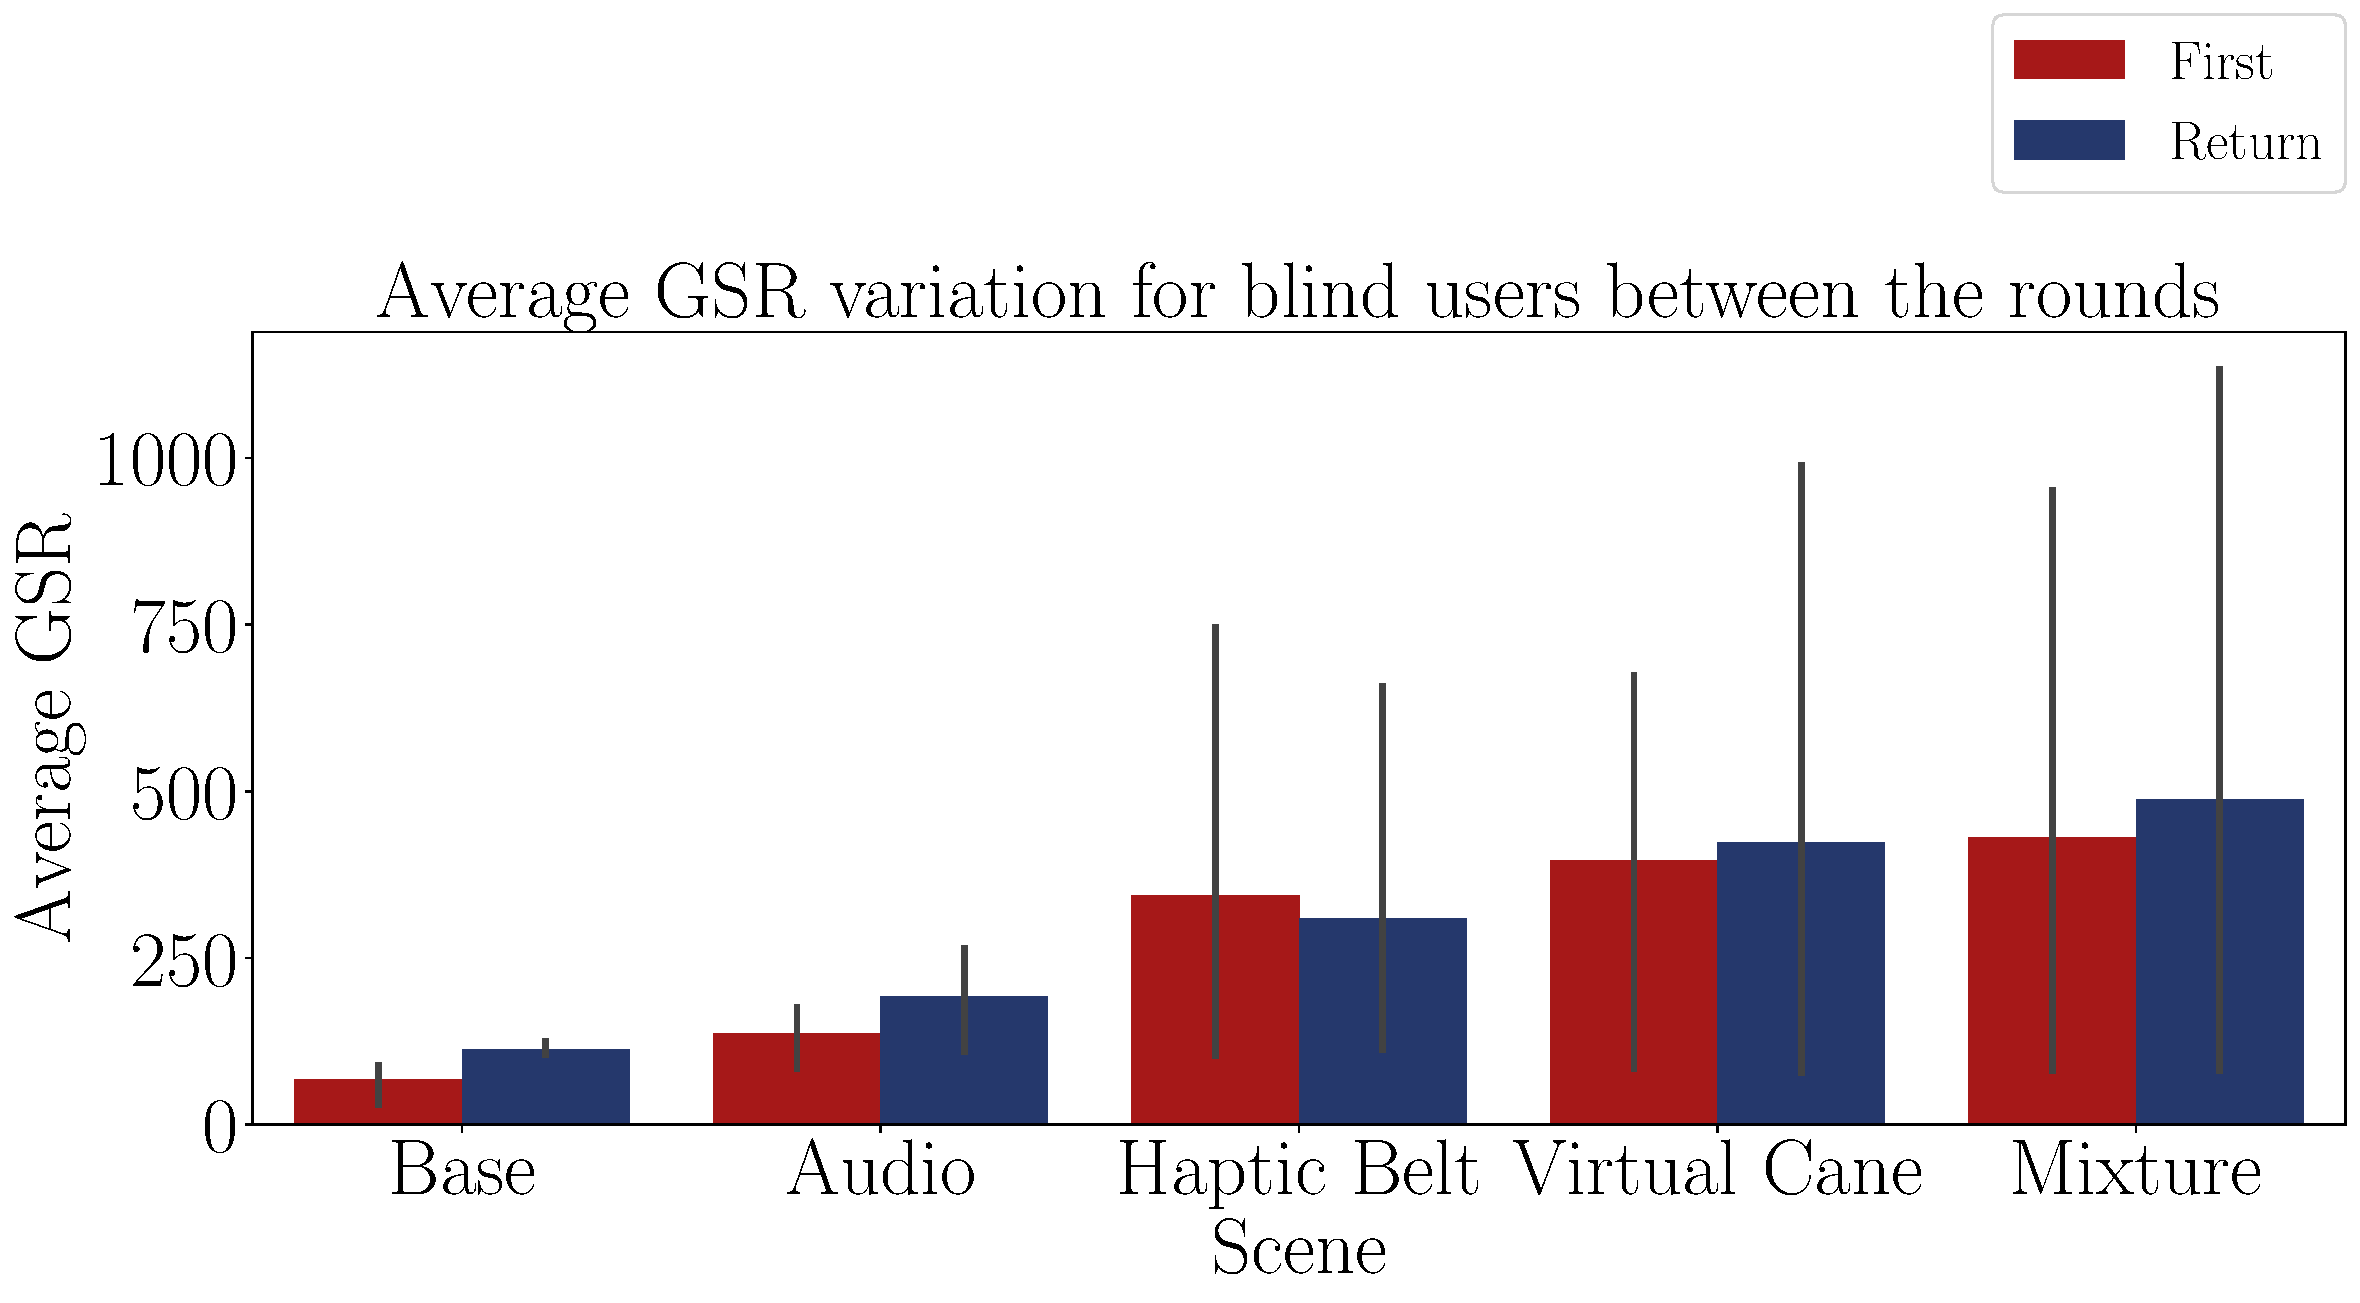
\includegraphics[width = \textwidth]{Resultados/GSR/Figuras/pdf/barplot_gsr_avg_5_scene_blind.pdf}
    \caption{Barplot of the average SDNN of the blind participants on each method.}
    \label{fig:barplot_gsr_avg_5_scene_blind}
\end{figure}

Figure \ref{fig:boxplot_gsr_avg_blind_scene} presents the boxplot of the percentual variation in the skin conductance for each method. The base method has the lowest variation among all methods. Also, the introduction of vibration increases the method variance. Figure \ref{fig:boxplot_gsr_avg_blind_rounds} presents the GSR grouped by the rounds. In this case, there is no apparent difference between the rounds.

\begin{figure}[!htb]
    \centering
    \begin{minipage}{0.45\textwidth}
        \centering
        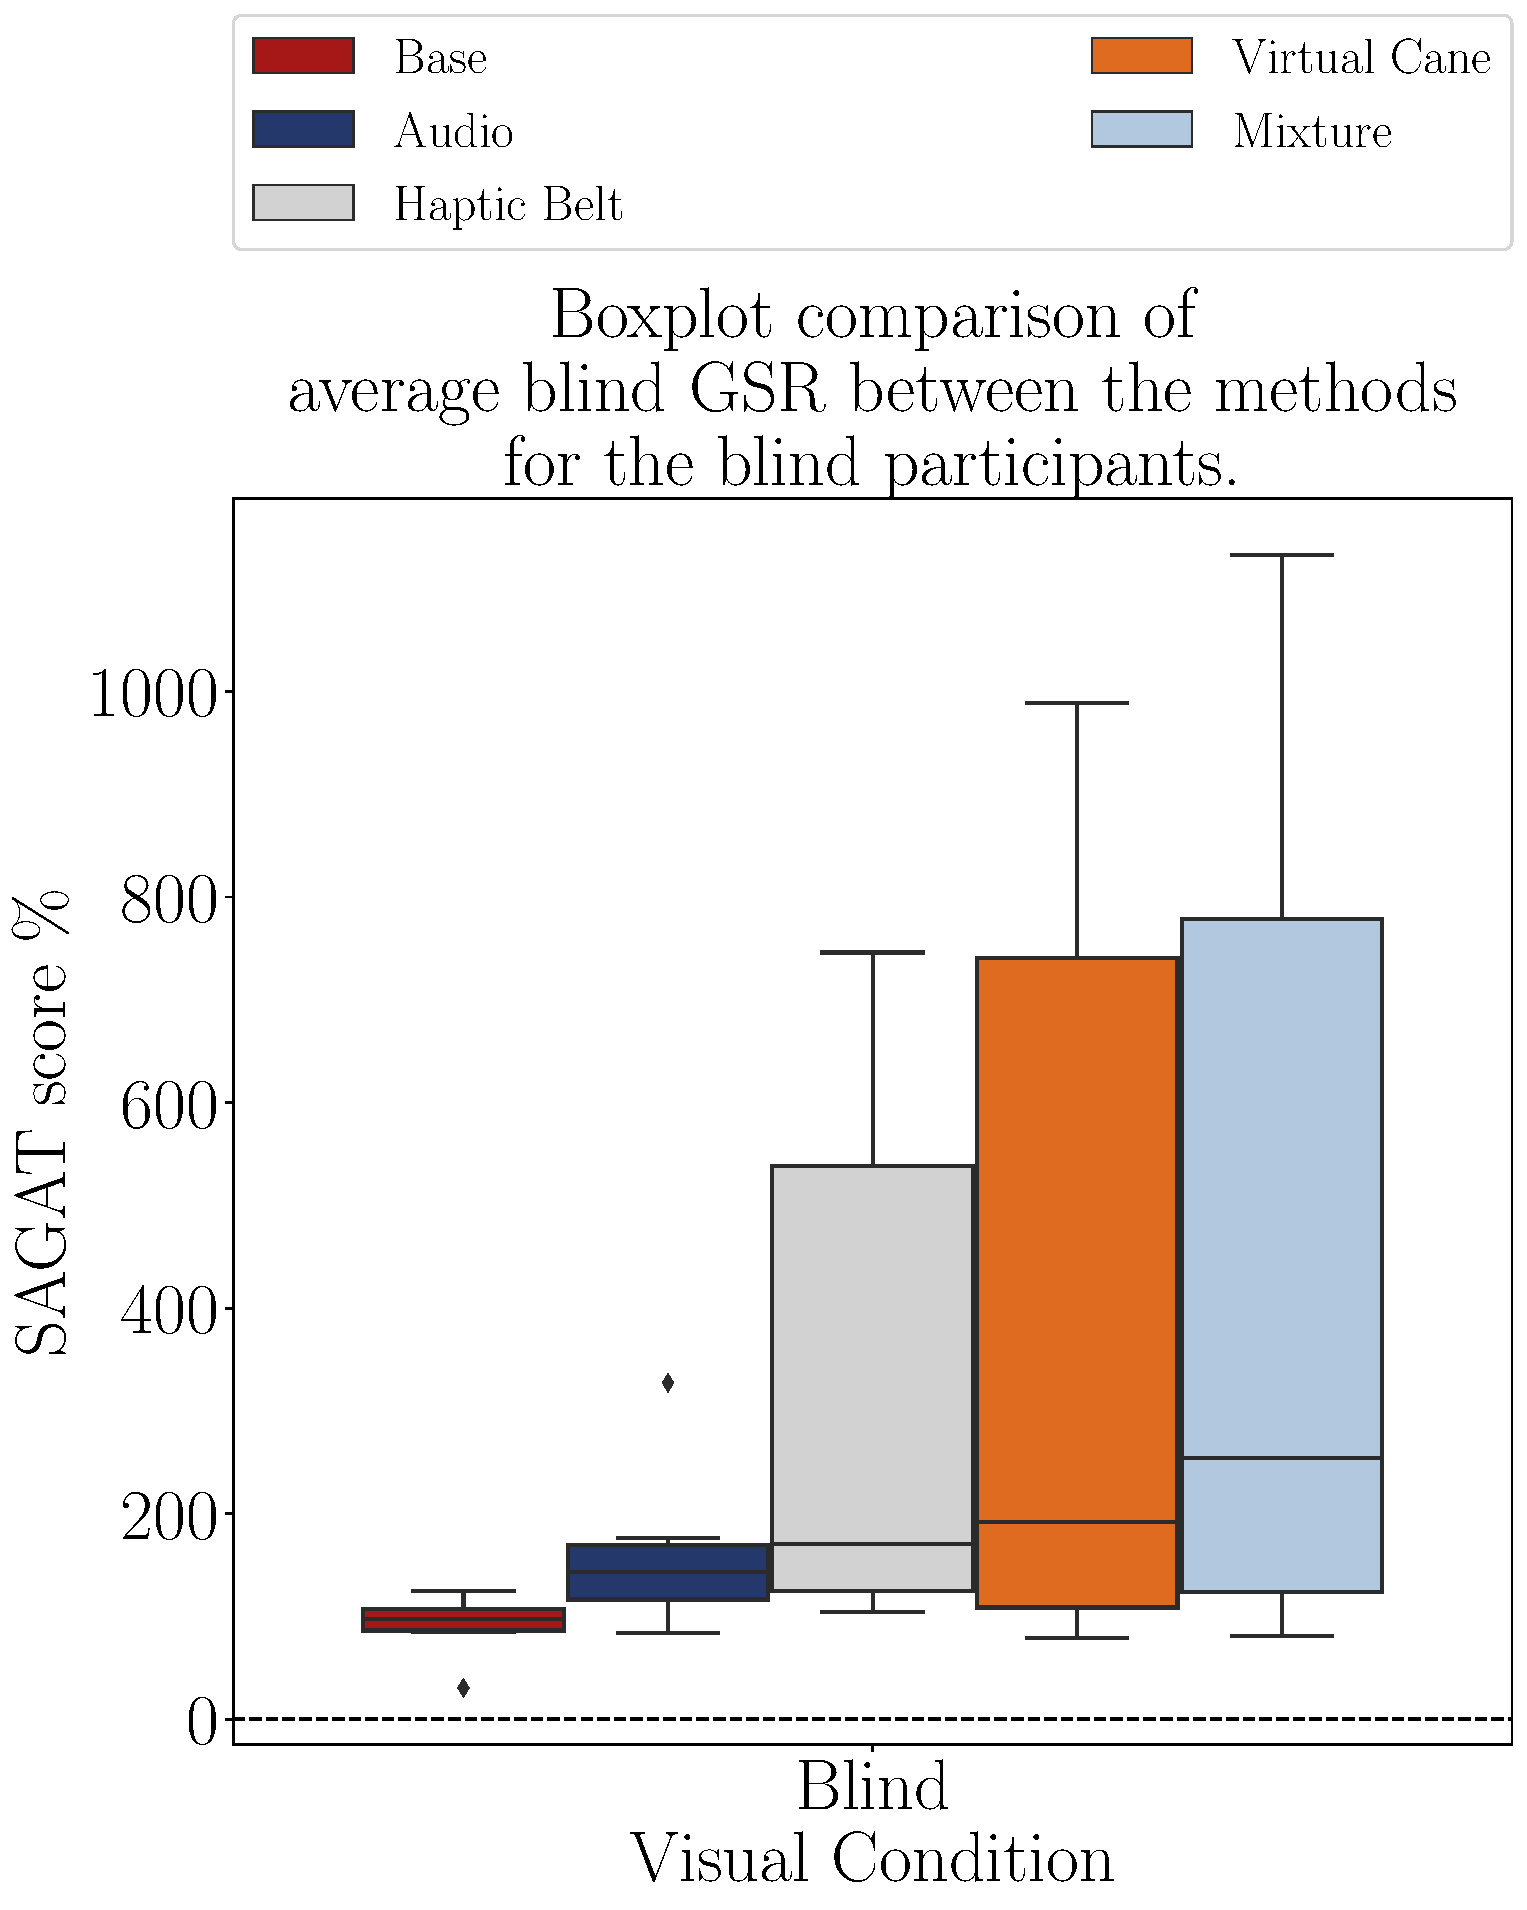
\includegraphics[width = \textwidth]{Resultados/GSR/Figuras/pdf/boxplot_gsr_avg_blind_scene.pdf}
        \caption{Boxplot of the GSR of the blind participants grouped by the methods.}
        \label{fig:boxplot_gsr_avg_blind_scene}
    \end{minipage}
    \begin{minipage}{0.075\textwidth}
        \hfill
    \end{minipage}
    \begin{minipage}{0.45\textwidth}
        \centering
        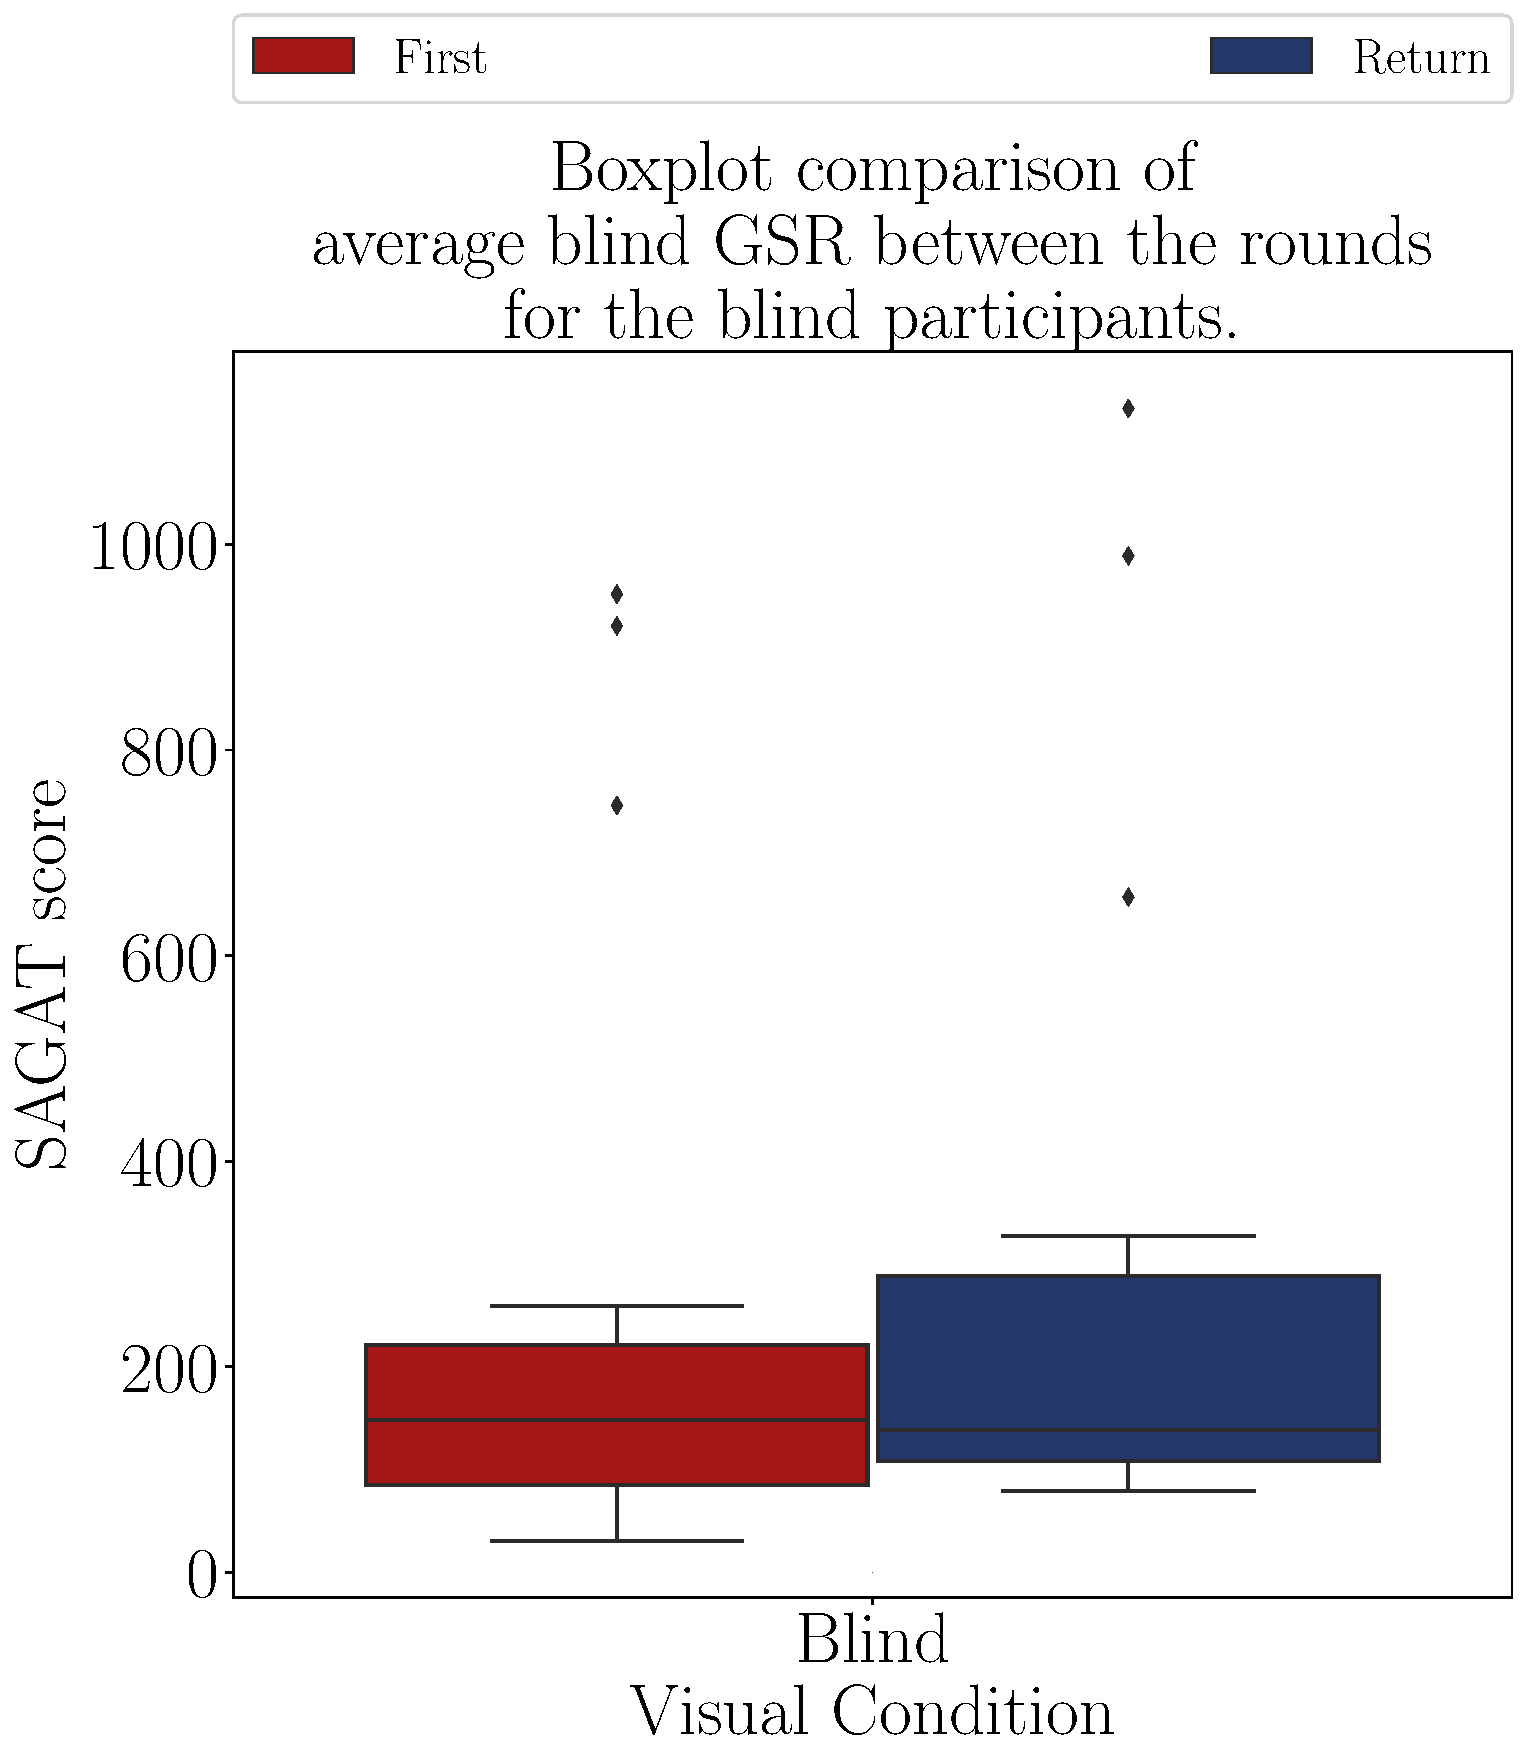
\includegraphics[width = \textwidth]{Resultados/GSR/Figuras/pdf/boxplot_gsr_avg_blind_rounds.pdf}
        \caption{Boxplot of the GSR of the blind participants grouped by the rounds.}
        \label{fig:boxplot_gsr_avg_blind_rounds}
    \end{minipage}
\end{figure}

Figures \ref{fig:qqplot_gsr_two_way_blind} and \ref{fig:residplot_gsr_two_way_blind} shows the QQ plot and the residual distribution. Table \ref{tab:blocanova_gsr_two_way_blind} shows the ANOVA test p-value for the GSR percentual variance. Although the p-value for the method is not below the threshold of 0.05, it is close to it, indicating that probably the GSR is affected by it. 

\begin{figure}[!htb]
    \centering
    \begin{minipage}{0.45\textwidth}
        \centering
        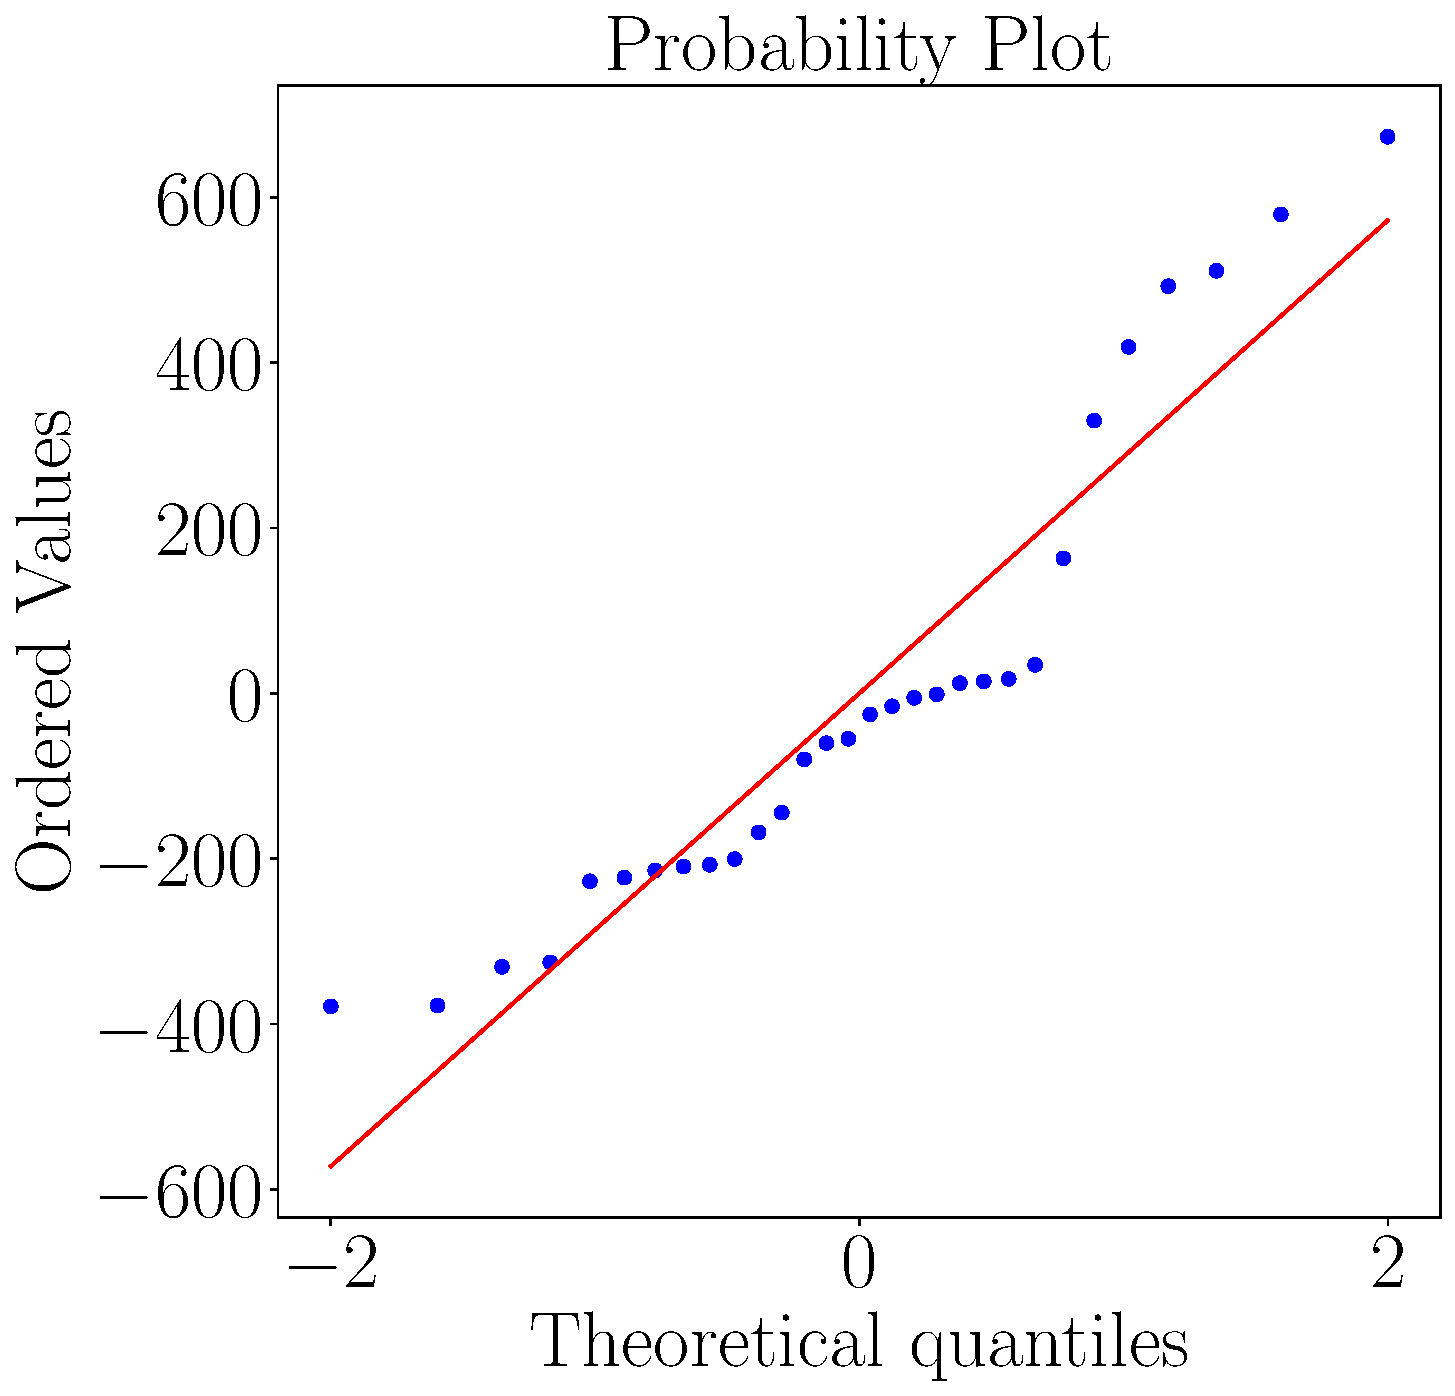
\includegraphics[width = \textwidth]{Resultados/GSR/Figuras/pdf/qqplot_gsr_two_way_blind.pdf}
        \caption{QQ plot of the SDNN of the blind participants on each method.}
        \label{fig:qqplot_gsr_two_way_blind}
    \end{minipage}
    \begin{minipage}{0.075\textwidth}
        \hfill
    \end{minipage}
    \begin{minipage}{0.45\textwidth}
        \centering
        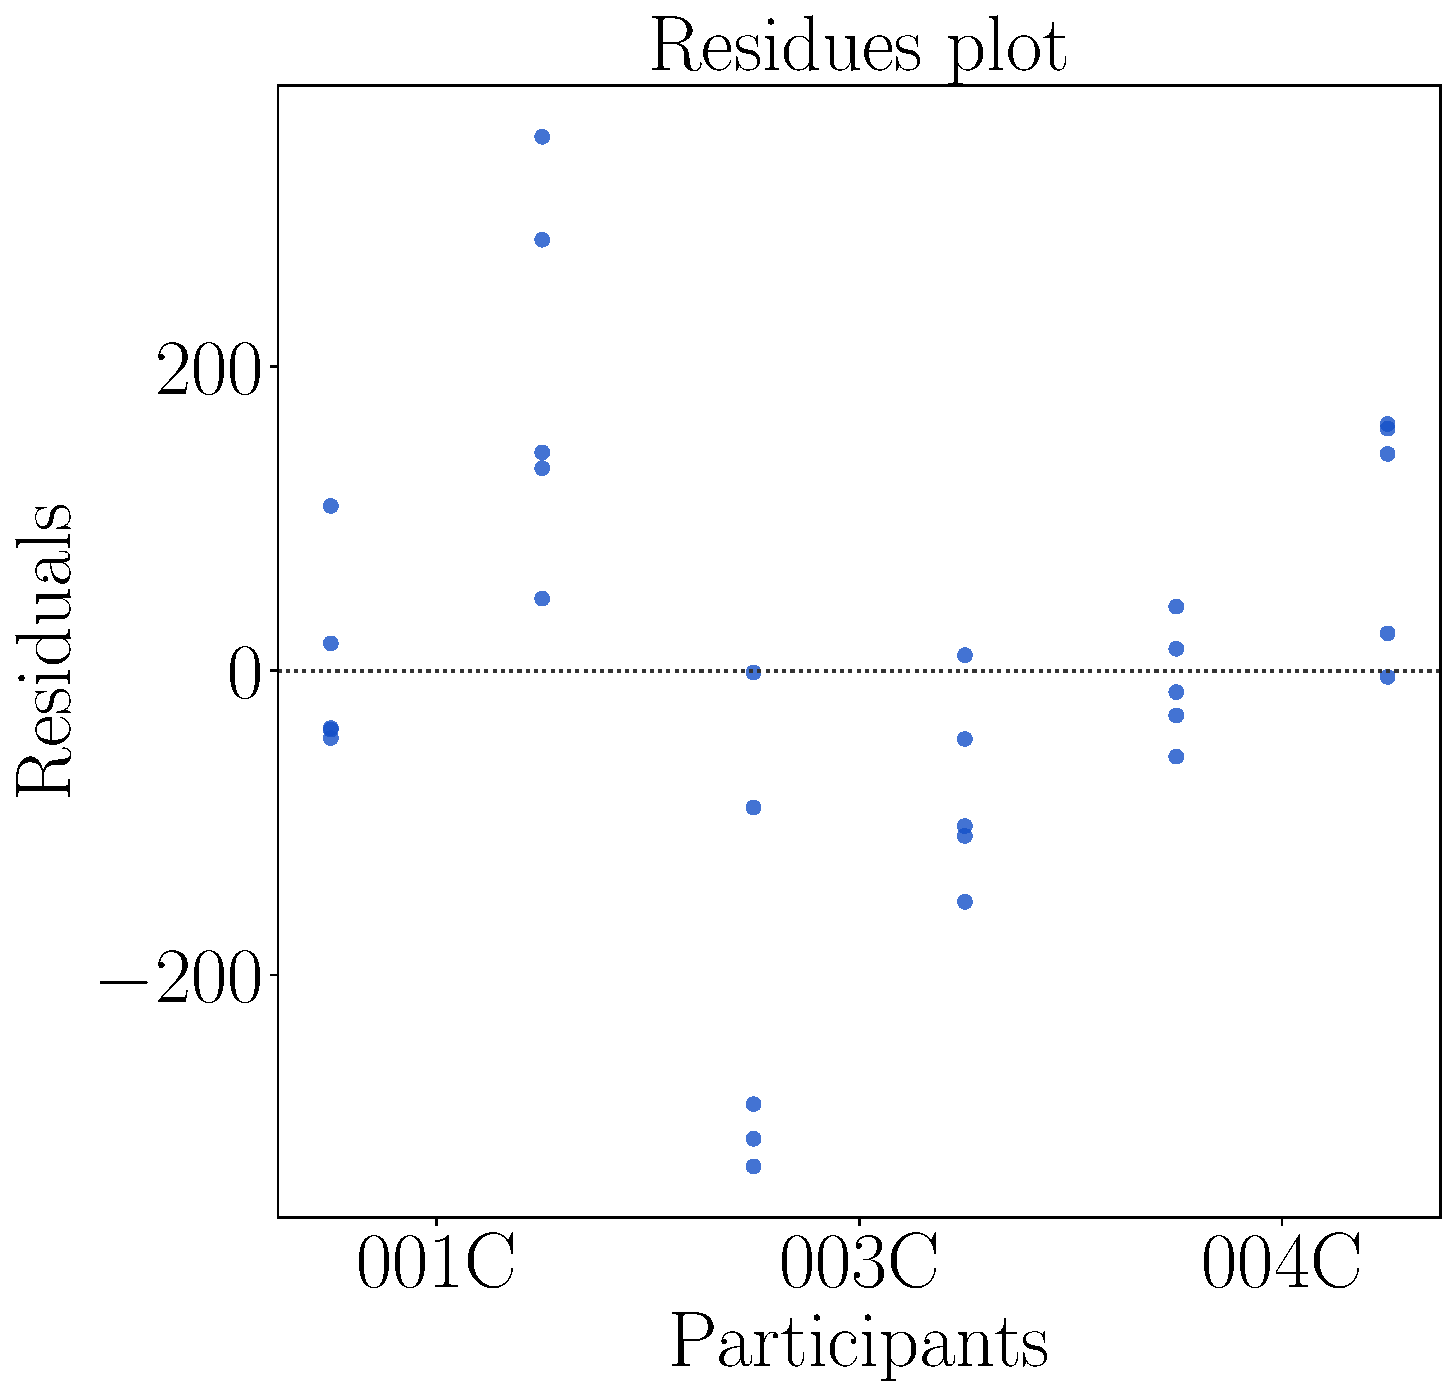
\includegraphics[width = \textwidth]{Resultados/GSR/Figuras/pdf/residplot_gsr_two_way_blind.pdf}
        \caption{Residual plot of the SDNN of the blind participants on each method.}
        \label{fig:residplot_gsr_two_way_blind}
    \end{minipage}
\end{figure}


\begin{table}[!htb]
\centering
\caption{Anova p-value for the mental demand average on each method for blinded users.}
\label{tab:blocanova_gsr_two_way_blind}
\begin{tabular}{lrrrrl}
\toprule
          Source & P-Value \\
\midrule
    \    Methods &   0.051 \\
     \    Rounds &   0.722 \\
\    Interaction &   0.996 \\
\bottomrule
\end{tabular}
\end{table}




\FloatBarrier

